\documentclass[11pt,a4paper]{article}
\usepackage[margin=22mm,headheight=16pt,footskip=12mm]{geometry}
\usepackage[T1]{fontenc}
\usepackage[utf8]{inputenc}
\usepackage{lmodern,amsmath,amssymb,graphicx,xcolor,booktabs,longtable,array,tabularx}
\usepackage{tikz,float,caption,fancyhdr,titlesec,url,lscape}
\usetikzlibrary{arrows.meta,positioning,calc}
\definecolor{navy}{HTML}{16324F}
\definecolor{teal}{HTML}{007F86}
\definecolor{pale}{HTML}{EAF5F5}
\definecolor{ink}{HTML}{243646}
\definecolor{amber}{HTML}{A45C13}
\pdfinfo{/Title (Environment-Aware Exact Inverse-GPR Fuel Control) /Author (T-MATS Controller Development Study)}
\urlstyle{tt}
\setlength{\parindent}{0pt}
\setlength{\parskip}{5pt plus 1pt minus 1pt}
\setlength{\emergencystretch}{2em}
\widowpenalty=10000\clubpenalty=10000
\linespread{1.05}
\titleformat{\section}{\Large\sffamily\bfseries\color{navy}}{\thesection}{.7em}{}
\titleformat{\subsection}{\large\sffamily\bfseries\color{teal}}{\thesubsection}{.7em}{}
\titlespacing*{\section}{0pt}{19pt}{8pt}
\titlespacing*{\subsection}{0pt}{13pt}{5pt}
\captionsetup{font=small,labelfont={bf,color=navy},skip=8pt}
\pagestyle{fancy}\fancyhf{}
\fancyhead[L]{\small\sffamily\color{navy}INVERSE-GPR VIRTUAL-FUEL PI}
\fancyhead[R]{\small\sffamily T-MATS control study}
\fancyfoot[L]{\scriptsize\color{ink}Altitude / ISA extension with fixed PI gains}
\fancyfoot[R]{\small\thepage}
\renewcommand{\headrulewidth}{.3pt}
\tikzset{block/.style={draw=navy!55,fill=navy!3,rounded corners=3pt,minimum height=.92cm,align=center,font=\sffamily\small,inner sep=5pt},
gp/.style={block,draw=teal,fill=pale},plant/.style={block,draw=navy,fill=navy!12},
sum/.style={circle,draw=navy,minimum size=.68cm,fill=white,font=\large},
arr/.style={-{Latex[length=2.2mm]},draw=navy,line width=.65pt},
lab/.style={font=\small,fill=white,inner sep=2pt},
note/.style={font=\small\sffamily,text=ink,align=left}}
\begin{document}
\begin{titlepage}
\color{navy}\sffamily
{\small T-MATS / EXACT GPR / ENVIRONMENTAL TRANSFER}\par\vspace{18mm}
{\fontsize{29}{35}\selectfont\bfseries Environment-Aware\\Inverse-GPR\\Fuel Control\par}
\vspace{9mm}{\Large Altitude and ISA extension, fixed PI gains,\\and disturbance-response comparison\par}
\vspace{10mm}\color{teal}\rule{\linewidth}{1.2pt}\color{navy}\vspace{8mm}
\begin{tabular}{@{}ll}
Environment grid & 5 altitudes $\times$ 7 ISA departures\\[5pt]
Inverse model & Exact GPR: $N,\dot N,T_{t2},P_{t2}\rightarrow W_f$\\[5pt]
Data & 1,400 training points / 200 held-out test points\\[5pt]
Virtual-fuel PI & $K_p=2,\ K_i=30\ \mathrm{s}^{-1}$\\[5pt]
Requested transfer test & 4000 m, ISA+5, 9500 rpm, 10\% shaft-load steps\\[5pt]
Report date & 14 September 2026
\end{tabular}
\par\vspace{10mm}\normalfont\color{ink}
\textbf{Measured result.} At 4000 m, ISA+5 and 9500 rpm, base PI achieved speed RMSE 2.531 rpm; the fixed-gain inverse-GPR PI plus feedforward achieved 1.819 rpm. The corresponding fuel-ringing scores were 2.030 and 3.817 lbm/s. Both controllers passed the full-run numerical and surge-margin checks.

This report derives the new controller inputs and regression, documents the data split, and examines speed accuracy, fuel ringing, recovery and model-domain limitations. It includes 73 controller trajectories: paired comparisons across 35 environmental combinations, plus three methods at the requested off-grid condition.

\vfill Some cold, high-altitude conditions exceed the original compressor map's corrected-speed range. Those simulation results are explicitly flagged and do not establish physical engine validity outside the component maps.
\end{titlepage}
\tableofcontents\clearpage

\section{Objective and experimental scope}
The previous inverse controller represented nominal fuel as a function of shaft speed and acceleration at one ambient condition. Changing altitude changes inlet pressure and density; changing ISA departure changes inlet temperature and corrected shaft speed. The same physical speed and acceleration can therefore require different fuel rates. A two-input inverse cannot distinguish these environments.

The extension uses one global four-input exact Gaussian-process regression, evaluated twice online: once for desired motion and once for measured motion. These are the setpoint and feedback inverse models in the control diagram; they share one fitted posterior rather than independently fitted regressions. The previous selected virtual-fuel PI gains are frozen. The base speed PI gains are also unchanged. No gain scheduling is enabled and the requested transfer test is not used to select gains, kernel parameters or training points.

\begin{table}[H]\centering\small
\begin{tabularx}{\linewidth}{@{}lX@{}}\toprule Item & Definition\\\midrule
Altitude grid & $0,2500,5000,7500,10000$ m\\
ISA departures & $0,-10,+10,+20,-20,+30,-30$ K relative to the standard-day temperature at altitude\\
Training design & 40 valid, input-space-selected points per condition; 1,400 total\\
Held-out test & Exactly 200 observations, selected after freezing the posterior\\
Grid controller tests & Base PI and inverse-GPR PI plus FF, both at 9500 rpm with 10\% load steps\\
Off-grid controller test & 4000 m, ISA+5: base PI, inverse-GPR PI plus FF, and inverse-GPR PI without FF\\
Sampling & 0.015 s; speed-sensor time constant 0.05 s; acceleration-filter time constant 0.03 s\\
Limits & Fuel command $0.2\leq W_f\leq4$ lbm/s; existing speed-governor rate 150 rpm/s\\
Noise & No added sensor noise; deterministic simulated plant signals\\\bottomrule
\end{tabularx}\caption{Scope and frozen implementation settings.}\end{table}

The 4000 m/ISA+5 pair is absent from the environmental training grid. This is an interpolation test in environmental coordinates, not evidence of extrapolation beyond the requested altitude/temperature envelope. The load-disturbance trajectory is also separate from the unloaded identification experiments.

\subsection{What a 10\% disturbance means}
The disturbance is a physical shaft-power extraction, not a fuel-command perturbation or a percentage of speed. Each environmental condition first receives an unloaded base-PI preparation run. Its mean turbine power over absolute time 55--60 s is frozen as $P_{t,0}$. Both controllers then receive
\begin{equation}
P_L(t)=0.10P_{t,0}\,s(t),\qquad
J\dot\omega=\tau_t-\tau_c-\frac{P_L}{\omega},\qquad N=\frac{60}{2\pi}\omega.
\end{equation}
The same load amplitude and timing are used for both methods within a condition. The controllers do not receive the load schedule. Because $P_{t,0}$ changes with environment, percentages are comparable but absolute horsepower is not identical across altitudes.

\clearpage
\section{Environment and inlet-state inputs}
The T-MATS ambient block takes altitude in feet, a temperature departure in degrees Fahrenheit, and Mach number. This study retains Mach zero and the existing inlet pressure recovery. User-specified altitude is converted as $h_{\rm ft}=h_{\rm m}/0.3048$; a temperature difference of one kelvin is 1.8 degrees Fahrenheit. The existing tabulated standard atmosphere is retained:
\begin{equation}
T_s(h,\Delta T)=T_{\rm ISA,table}(h)+\Delta T,\qquad
P_s(h,\Delta T)=P_{\rm ISA,table}(h).
\end{equation}
Thus ISA departures change temperature at a fixed pressure altitude. This is the implemented T-MATS convention; a separate nonstandard hydrostatic atmosphere is not constructed. Linear interpolation of the existing atmosphere tables is used, rather than replacing them with a different analytical atmosphere.

The regression inputs are the actual logged inlet station-2 \emph{total} temperature and pressure after the inlet block. They are converted from the native units:
\begin{equation}
T_{t2}[\mathrm K]=T_{t2}[{}^\circ\mathrm R]/1.8,
\qquad P_{t2}[\mathrm{kPa}]=6.894757293168\,P_{t2}[\mathrm{psia}].
\end{equation}
Using actual station measurements avoids confusing ambient static pressure with inlet total pressure. The controller samples both inlet signals with one sample of delay to keep the feedback interface causal. At the constant environmental condition during evaluation, this delay does not change their steady values.

\subsection{Preparation and initialization}
All runs begin at the inherited sea-level initial state. Altitude and ISA departure ramp from zero between absolute time 5 and 30 s. This avoids imposing an inconsistent high-altitude thermodynamic state on the inherited solver initialization. The speed request ramps from 10000 to 9500 rpm between 5 and 10 s. The inverse controller takes over at 45 s, after the environmental ramp; evaluation begins at 60 s. The handover time is a preparation change from the previous study, not a gain change. Performance is scored only after preparation, while full-run numerical checks also monitor startup.

At the requested transfer point the measured inlet values are
\begin{equation}
T_{t2}=267.1614\ \mathrm K,\qquad P_{t2}=60.64817\ \mathrm{kPa}.
\end{equation}
The unloaded reference turbine power is 15030.12 hp, so the applied disturbance is 1503.012 hp. These values come from the new trim simulation, not a reused sea-level power reference.

\subsection{Compressor-map domain}
The unchanged compressor map has normalized corrected-speed limits $[0.5,1.05]$. Its monitored coordinate is
\begin{equation}
N_{c,\rm map}=\frac{N}{10000\sqrt{T_{t2}/288.15}}.
\end{equation}
Cold inlet conditions increase corrected speed even if actual speed remains 9500 rpm. Inspection of the installed T-MATS interpolation routine shows that out-of-range coordinates are clamped to the map boundary and produce a warning. Consequently, convergence outside this range describes the boundary-clamped simulator, not a validated compressor characteristic. Map flags are kept separate from numerical acceptance. This specific coordinate check is not a comprehensive audit of every component map or every intermediate Newton iteration.

\clearpage
\section{Data generation and exact inverse regression}
\subsection{Unloaded identification experiments}
The 35 trajectories retain the full nonlinear T-MATS plant with zero external shaft extraction. After preparation, the base PI tracks a bounded multisine speed command, while small additive fuel excitation supplies additional acceleration variation. With $q=t-40$, the first design uses
\begin{align}
r(t)&=9500+150\sin(2\pi\,0.025q)+100\sin(2\pi\,0.065q),\\
\delta W_f(t)&=0.025\sin(2\pi\,0.7q)+0.012\sin(2\pi\,1.13q).
\end{align}
Training eligibility is restricted to absolute time $45\leq t<90$ s and $9000\leq N\leq10000$ rpm. In each environment, 40 samples are selected by deterministic farthest-point coverage in standardized speed/acceleration space. Environmental balance is imposed by the equal per-condition count, and measured fuel values are not used to optimize the selection.

For the second excitation, beginning at 100 s, the speed amplitudes are 170 and 70 rpm at 0.031 and 0.081 Hz; fuel amplitudes are 0.023 and 0.010 lbm/s at 0.57 and 0.93 Hz. Held-out eligibility begins at 105 s. No training and test source rows overlap. The labels use the plant shaft acceleration and actual delivered fuel, not a numerical derivative of speed or the GP's own predictions.

The windows belong to different phases of the same environmental trajectories. They are held out from fitting but are temporally correlated simulation data, not 200 independent experimental replicates. The separate off-grid load test provides additional closed-loop evidence.

\subsection{Validity and the 200-point allocation}
Eligible rows require finite monitored signals, positive fuel, positive surge margin, maximum absolute flow residual at most $10^{-9}$, and fewer than 200 solver iterations. All 35 environments supplied 40 eligible training points. The 10000 m/ISA and 10000 m/ISA+10 trajectories supplied no valid held-out-window samples. Their failure is retained in the coverage table, and they receive no test predictions in the 200-point accuracy calculation.

After freezing the fitted posterior, the 200 observations were allocated across the 33 environments with valid held-out data: six per environment, plus one additional point in each of the first two eligible environments. Within each eligible window, unique rows were spread across time. This adjustment used numerical eligibility only; the posterior was not refitted and no prediction-error-based rejection was applied.

Of the selected observations, 396 training points and 52 test points exceed the monitored compressor corrected-speed range. They remain in this full-grid simulator-identification study but are model-domain flagged. The aggregate GP scores therefore measure agreement with the supplied simulator, including its boundary behaviour.

\begin{table}[H]\centering\small
\setlength{\tabcolsep}{5pt}
\begin{tabular}{@{}lrrrr@{}}\toprule
Variable & Train min & Train max & Test min & Test max\\\midrule
Speed (rpm) & 9264.2 & 9750.6 & 9282.4 & 9732.4\\
Acceleration (rpm/s) & -68.842 & 61.628 & -54.435 & 47.868\\
Inlet total temperature (K) & 193.25 & 318.15 & 193.25 & 318.15\\
Inlet total pressure (kPa) & 26.111 & 99.299 & 26.111 & 99.299\\
Fuel response (lbm/s) & 0.59733 & 3.1499 & 0.64387 & 3.0569\\
\bottomrule\end{tabular}\caption{Observed ranges. A rectangular range is not a guarantee of joint input coverage.}\end{table}


\clearpage
\subsection{Posterior derivation}
Let an observation be
\begin{equation}
\mathbf x_i=[N_i,\ a_i,\ T_{t2,i},\ P_{t2,i}]^{\mathsf T},\qquad y_i=W_{f,i}.
\end{equation}
Input and output standardization uses training data only:
\begin{equation}
z_{ij}=\frac{x_{ij}-\mu_{x,j}}{s_{x,j}},\qquad \tilde y_i=\frac{y_i-\mu_y}{s_y}.
\end{equation}
The model uses a zero basis mean in standardized response coordinates and an ARD squared-exponential covariance,
\begin{equation}
k(\mathbf z,\mathbf z')=\sigma_f^2\exp\left[-\frac12\sum_{j=1}^{4}\frac{(z_j-z'_j)^2}{\ell_j^2}\right].
\end{equation}
Four learned length scales allow different sensitivities to speed, acceleration, temperature and pressure. Hyperparameters, including response-noise standard deviation, are estimated by MATLAB's exact GP fitting method. Prediction also uses the exact method; no sparse active-set approximation is used~\cite{mathworks}.

With $K_{ij}=k(\mathbf z_i,\mathbf z_j)$, the exported posterior stores
\begin{equation}
LL^{\mathsf T}=K+\sigma_n^2I,\qquad
\boldsymbol\alpha=L^{-\mathsf T}L^{-1}\tilde{\mathbf y}.
\end{equation}
For a query $\mathbf x_*$, the inverse-fuel mean is
\begin{equation}
g(\mathbf x_*)=\mu_y+s_y\mathbf k_*^{\mathsf T}\boldsymbol\alpha.
\end{equation}
The latent and response uncertainty are
\begin{align}
\sigma_{\rm latent}^2(\mathbf x_*)&=s_y^2\max\{0,k(\mathbf z_*,\mathbf z_*)-\|L^{-1}\mathbf k_*\|^2\},\\
\sigma_{\rm response}^2(\mathbf x_*)&=\sigma_{\rm latent}^2(\mathbf x_*)+s_y^2\sigma_n^2.
\end{align}
The nominal 95\% response interval is $g\pm1.959964\sigma_{\rm response}$. These are standard conditional GP equations~\cite{gpml}. Exact refers to the posterior calculation, not an exact physical inverse, independent data, or guaranteed uncertainty calibration. Hyperparameter uncertainty, inlet-sensor uncertainty and uncertain component maps are not integrated.

For the fixed-gain online controller, only the mean coefficients are needed. The large Cholesky factor is retained in the saved offline model for standard-deviation predictions and omitted from the per-sample controller payload. Removing unused covariance storage leaves the posterior mean unchanged. Logged controller outputs are replayed against the full exported posterior as a numerical consistency check.

\clearpage
\section{Controller derivation and unchanged gains}
\subsection{Base speed PI}
The baseline retains the inherited PI path with speed error $e_N=r-N_s$:
\begin{equation}
u_P=K_{p,N}e_N+I_N,\qquad K_{p,N}=0.025,\quad K_{i,N}=0.05.
\end{equation}
The existing sensor, speed governor, fuel limits and plant remain in place. The observer compensation is disabled. The numerical values act on speed error in rpm, so their units differ from the virtual-fuel PI gains.

\subsection{Inverse-model setpoint and feedback}
The causal acceleration estimate is computed from sensed speed, with $T_s=0.015$ s and $\tau_a=0.03$ s:
\begin{equation}
\hat a_s[k]=p_a\hat a_s[k-1]+(1-p_a)\frac{N_s[k]-N_s[k-1]}{T_s},\qquad p_a=e^{-T_s/\tau_a}.
\end{equation}
Both GP branches receive the same sampled inlet measurements:
\begin{align}
v_r[k]&=g(r[k],0,T_{t2}[k-1],P_{t2}[k-1]),\\
v_y[k]&=g(N_s[k],\hat a_s[k],T_{t2}[k-1],P_{t2}[k-1]),\\
e_v[k]&=v_r[k]-v_y[k].
\end{align}
The acceleration setpoint is zero for these constant-speed disturbance experiments. The load is deliberately absent from the inverse input: the GP estimates the nominal unloaded fuel associated with motion, while feedback supplies the residual needed under shaft extraction.

\subsection{Fuel-domain PI plus GPR feedforward}
With the previous selected gains retained,
\begin{align}
u^*[k]&=v_r[k]+2e_v[k]+I_v[k],\\
u[k]&=\operatorname{sat}_{[0.2,4]}u^*[k],\\
I_v[k+1]&=I_v[k]+T_s\,30\,e_v[k]\,\gamma[k].
\end{align}
The conditional-integration gate $\gamma$ is one unless the error would drive an already saturated command farther beyond the relevant limit. Before handover, the residual integral tracks $u_P-v_r-2e_v$, giving a bumpless transition. The no-FF diagnostic omits $v_r$ from the command and uses the corresponding integral tracking offset.

At constant $r,T_{t2},P_{t2}$, the feedforward term $v_r$ is constant. Defining $I'_v=I_v+v_r$ transforms the FF command into the no-FF command with the same feedback gains. With compatible initialization, the responses should coincide apart from numerical and preparation differences. The measured maximum differences over the full target trajectories are 2.26e-10 rpm and 8.56e-12 lbm/s. This equivalence does not predict the outcome for changing speed references or changing environmental inputs.

\subsection{Why fixed numerical gains can behave differently}
Locally, at a fixed environment,
\begin{equation}
e_v\simeq g_N e_N+g_a\dot e_N,
\end{equation}
where $g_N$ and $g_a$ are derivatives of the learned inverse. Ignoring the sensor/filter for interpretation,
\begin{equation}
\left(K_p+\frac{K_i}{s}\right)(g_N+g_as)
=K_pg_as+(K_pg_N+K_ig_a)+\frac{K_ig_N}{s}.
\end{equation}
Thus virtual-fuel PI has derivative-like action on speed. Retraining the GP changes the local slopes, and altitude changes the plant, even when $K_p$ and $K_i$ are fixed. The earlier ringing reduction at sea level is not automatically preserved. The shared inlet measurements cancel their common first-order contribution in the difference near the setpoint, but they change the operating-point slopes and the feedforward value. This is environmental model conditioning, not explicit uncertainty gain scheduling.

\section{Held-out inverse-model results}
\begin{table}[H]\centering\small
\setlength{\tabcolsep}{5pt}
\begin{tabular}{@{}lr@{}}\toprule
Metric & Value\\\midrule
Training observations & 1400\\
Held-out observations & 200\\
Training environments & 35\\
Represented held-out environments & 33\\
Fuel RMSE (lbm/s) & 0.00161248\\
Fuel MAE (lbm/s) & 0.000906799\\
Maximum absolute error (lbm/s) & 0.00780312\\
$R^2$ & 0.9999918\\
Nominal 95\% interval coverage & 93.5\%\\
Maximum exported-mean discrepancy (lbm/s) & 5.72e-12\\
Maximum exported-SD discrepancy (lbm/s) & 8.91e-13\\
\bottomrule\end{tabular}\caption{Validation of the frozen exact inverse GP. Export discrepancies compare the Cholesky implementation with MATLAB predict.}\end{table}

The small fuel prediction error supports the four-input representation for this simulator and sampled data. The nominal interval coverage is below 95\%, so the reported response standard deviation should not be treated as a calibrated physical confidence bound. Test observations share deterministic trajectories, and some lie beyond the compressor speed-map range. A high $R^2$ partly reflects the large fuel variation across environmental conditions; the absolute fuel error and the separate closed-loop trial are more informative for controller use.

The two missing 10000 m validation conditions are a limitation of the test coverage, not zero-error cases. No accuracy claim is made for their rejected held-out windows. The GP has training observations at those conditions, but its behaviour under the comparison disturbance still has to be judged independently.
\begin{figure}[H]\centering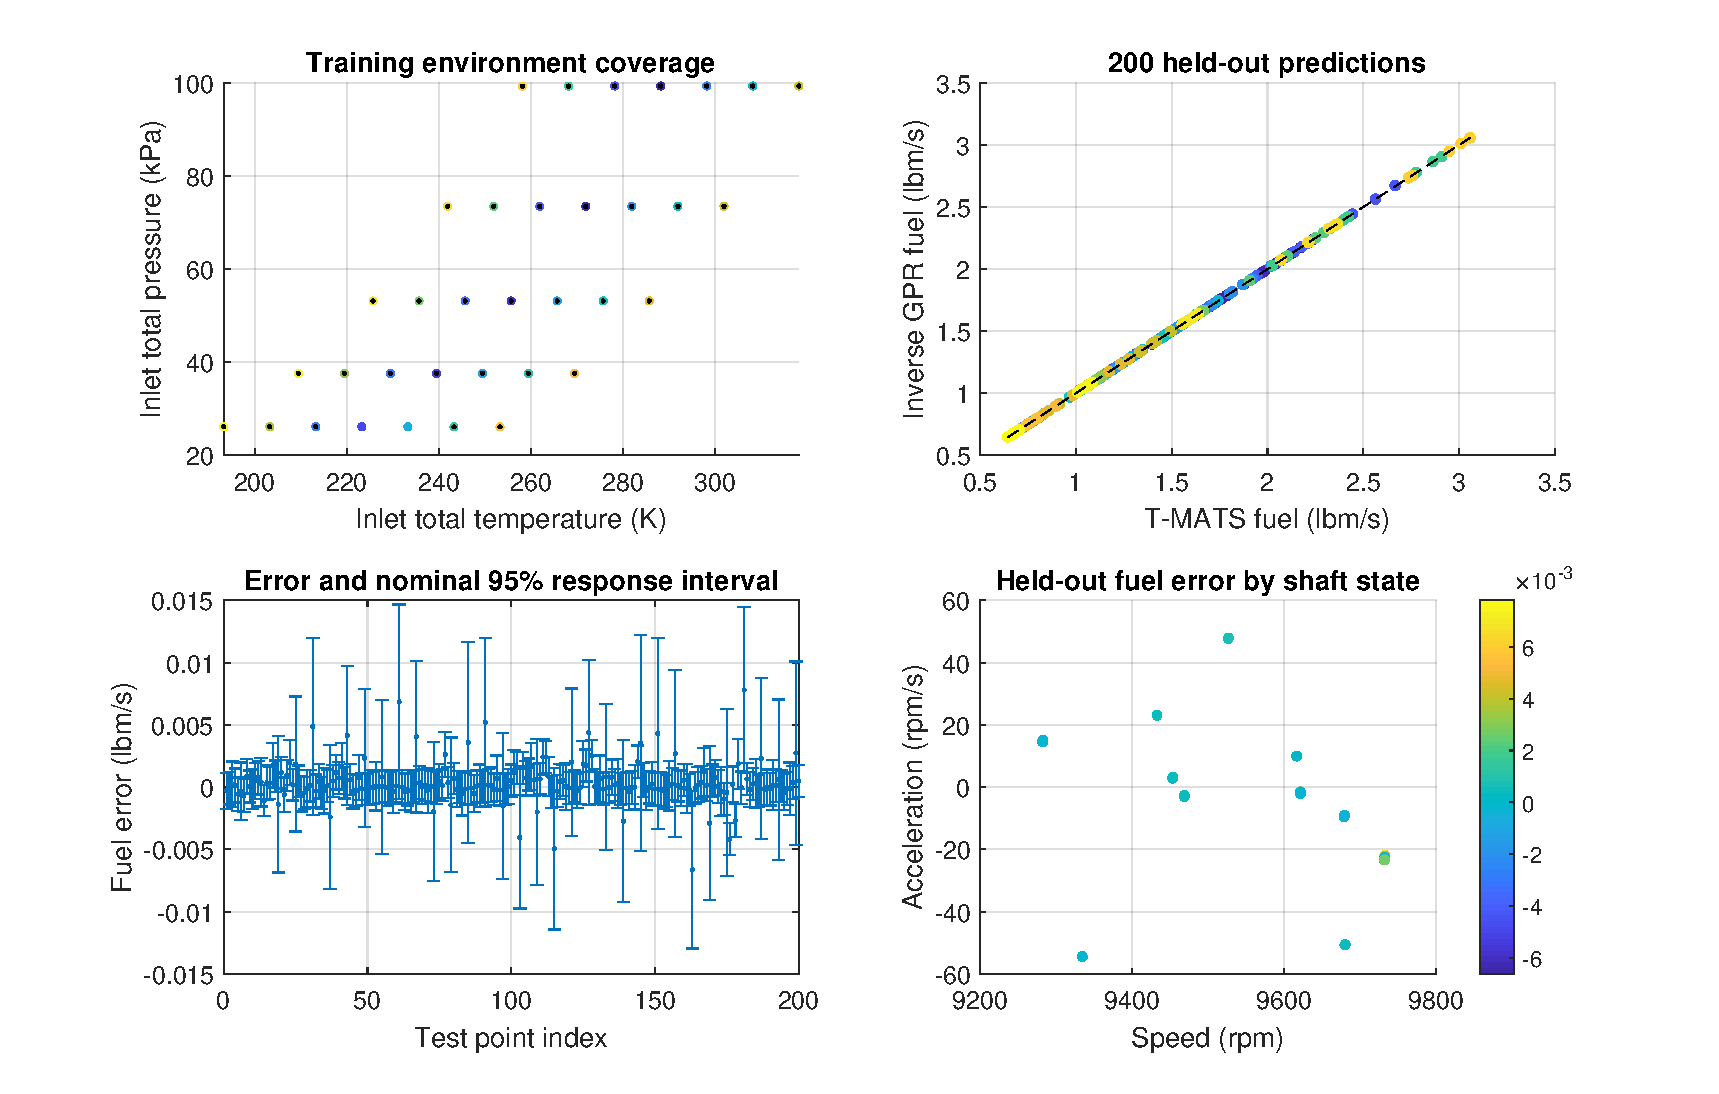
\includegraphics[width=\linewidth]{gpr_validation.pdf}\caption{Four-input coverage and held-out validation. Response intervals include the fitted noise variance; they do not quantify compressor-map uncertainty.}\end{figure}


\clearpage
\section{Response metrics and scoring rules}
The evaluation interval is absolute time 60--150 s. Let $e[k]=N[k]-9500$ and let $\mathcal E$ be its sample indices:
\begin{equation}
\mathrm{RMSE}_N=\sqrt{\frac1{|\mathcal E|}\sum_{k\in\mathcal E}e[k]^2},\qquad
\mathrm{IAE}_N=T_s\sum_{k\in\mathcal E}|e[k]|.
\end{equation}
These are speed tracking metrics over the complete 90 s interval, including quiet portions. Peak absolute error complements RMSE by exposing the largest transient.

\subsection{Fuel ringing}
For each load edge, take the two seconds following the edge. The ringing score removes the net monotonic fuel movement from total variation:
\begin{equation}
R_j=\max\left(0,\sum_{k\in\mathcal W_j}|W_f[k+1]-W_f[k]|-
|W_f[k_{j,\rm end}]-W_f[k_{j,\rm start}]|\right),\qquad R=\sum_{j=1}^{6}R_j.
\end{equation}
Its units are lbm/s. Zero means no excess reversal within the selected window, not zero fuel use. It is not integrated fuel mass and is not a frequency-domain oscillation measure. The largest two-second peak-to-peak fuel range and largest sampled fuel slew are also tabulated. All methods use identical windows and sampling.

\subsection{Recovery to the requested 1\% speed window}
The recovery band is relative to the 9500 rpm setpoint:
\begin{equation}
|N-9500|\leq0.01\times9500=95\ \mathrm{rpm}.
\end{equation}
For each event, recovery is measured from the load edge to the first sample after the last band violation, with the response required to remain inside until the next event (or end of evaluation). A response that never leaves the band receives zero. If it has not recovered by the next edge, it is marked NR. The general performance table reports the worst of six events.

A zero 1\% recovery can coexist with visible speed droop and fuel ringing, because $\pm95$ rpm is a broad band for these disturbances. A supplementary $\pm0.1$ rpm recovery criterion uses the same definition and reveals finer settling differences. This additional measure does not replace the user's requested metric.

\subsection{Acceptance and map qualification}
Full-run acceptance requires all numerical validity checks described above and maximum pre-test speed error below 0.1 rpm over 55--60 s. A rejected full run receives no RMSE, ringing or recovery score; its trace and failure time are retained. The separate compressor corrected-speed flag identifies simulations that rely on clamped map coordinates. Passing numerical checks or this one map-coordinate check alone is not a claim of full physical envelope validation.

\clearpage
\section{Requested case: 4000 m, ISA+5, 9500 rpm}
The load switches on at evaluation times 10.005, 30 and 60 s, and off at 15, 40.005 and 75 s. This repeats the earlier pulse convention at the requested 10\% amplitude. Each method starts from the same inherited plant state and uses the same preparation and disturbance schedules.

\begin{table}[H]\centering\small
\setlength{\tabcolsep}{5pt}
\begin{tabular}{@{}llrrr@{}}\toprule
Metric & Unit & P & VF & V\\\midrule
Speed RMSE & rpm & 2.53 & 1.82 & 1.82\\
Peak absolute speed error & rpm & 21.6 & 13.4 & 13.4\\
Integral absolute speed error & rpm s & 53.5 & 61.3 & 61.3\\
Fuel ringing, excess TV & lbm/s & 2.03 & 3.82 & 3.82\\
Largest 2 s fuel range & lbm/s & 0.586 & 0.64 & 0.64\\
Largest event-window fuel slew & lbm/s$^2$ & 4.67 & 10.6 & 10.6\\
Recovery to 1\% speed band & s & 0 & 0 & 0\\
Recovery to 0.1 rpm band & s & 2.46 & NR & NR\\
Minimum surge margin & \% & 9.01 & 8.73 & 8.73\\
Peak fuel & lbm/s & 2.13 & 2.15 & 2.15\\
Time at a fuel limit & \% & 0 & 0 & 0\\
Outside GP input rectangle & \% & 0 & 0.5 & 0.5\\
Outside compressor speed-map range & \% & 0 & 0 & 0\\
\bottomrule\end{tabular}\caption{Requested off-grid disturbance case. P: base PI; VF: inverse-GPR PI plus FF; V: inverse-GPR PI without FF. Gains are unchanged. Recovery is the worst of six events.}\end{table}

The new inverse controller changes RMSE by -28.2\% and fuel ringing by +88.0\% relative to base PI. Its worst recovery to the supplementary 0.1 rpm band is not reached before the next event in the first pulse, compared with 2.46 s for base PI. The minimum surge margins are 8.73\% and 9.01\%, respectively. These metrics describe different aspects of the transient; a smaller speed RMSE alone does not establish a better fuel command.

The inverse controller's first loaded interval lasts only 4.995 s, slightly shorter than its roughly 5.10 s recovery to the 0.1 rpm band on the longer loaded intervals. Its NR entry therefore does not mean permanent loss of regulation: the last unloaded tail reaches approximately 9500.0000--9500.0011 rpm over absolute time 145--150 s. Base PI reaches the tight band in about 2.42--2.46 s for all six events. The inverse controller also leaves the training acceleration range for about 0.50\% of evaluation samples; its speed and environmental inputs remain inside their observed training ranges.

No uncertainty schedule is involved. The comparison measures transfer of fixed gains through the newly trained, environmentally conditioned inverse. It does not compare separately optimized gains at the new altitude.

\clearpage
\subsection{Full time-domain response}
\begin{figure}[H]\centering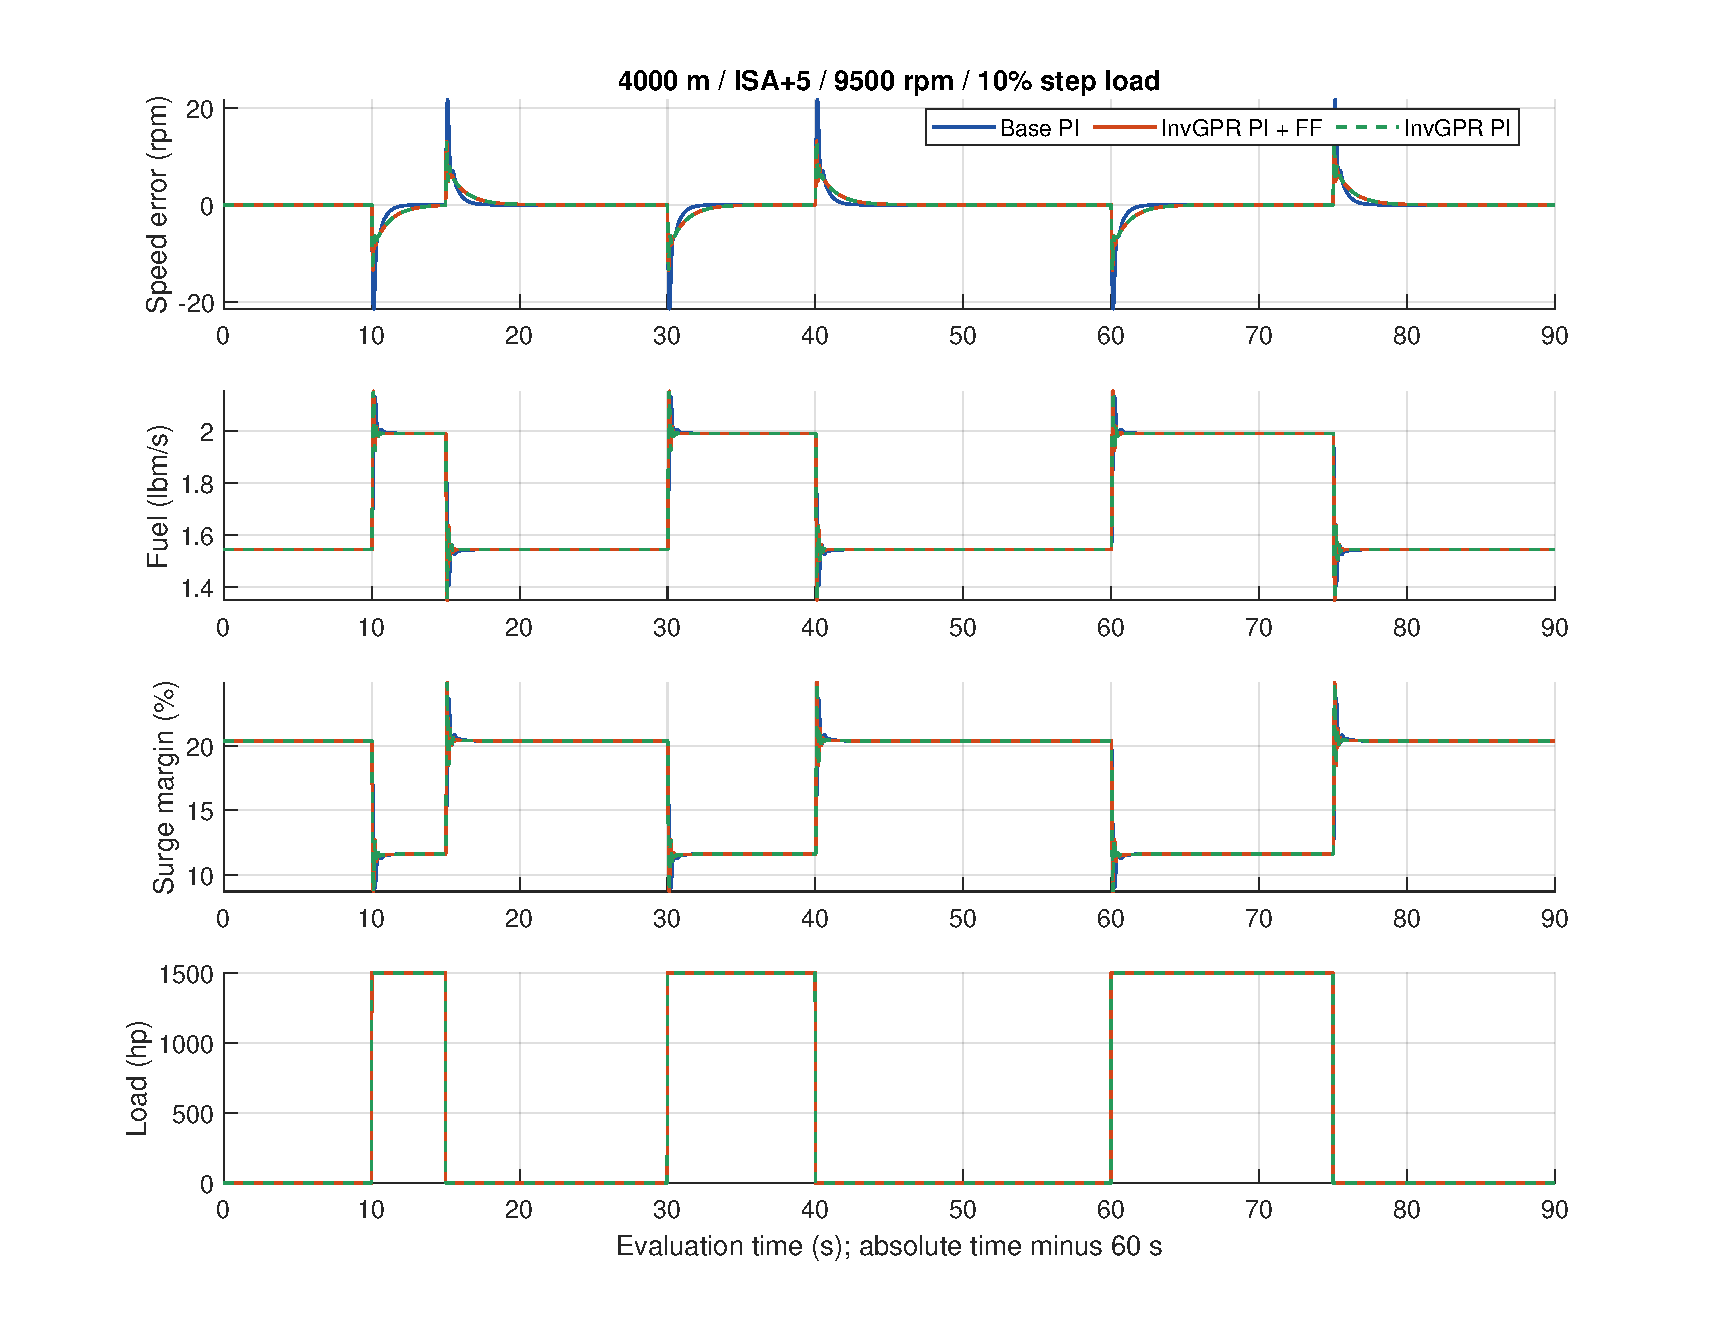
\includegraphics[width=\linewidth]{target_overview.pdf}\caption{Full requested disturbance comparison. The reference remains 9500 rpm. The three extracted-power pulses have different durations but the same amplitude. The inverse curves may overlap.}\end{figure}

The overview gives the speed-error scale, physical fuel levels, surge margin and the applied load on a common time axis. Detailed windows on the following pages prevent the 90 s view from hiding fuel reversals or small settling tails. The no-FF inverse case is included as a diagnostic of the constant-feedforward equivalence, rather than counted as a distinct improvement when its curve overlaps.

\clearpage
\subsection{First application and removal}
\begin{figure}[H]\centering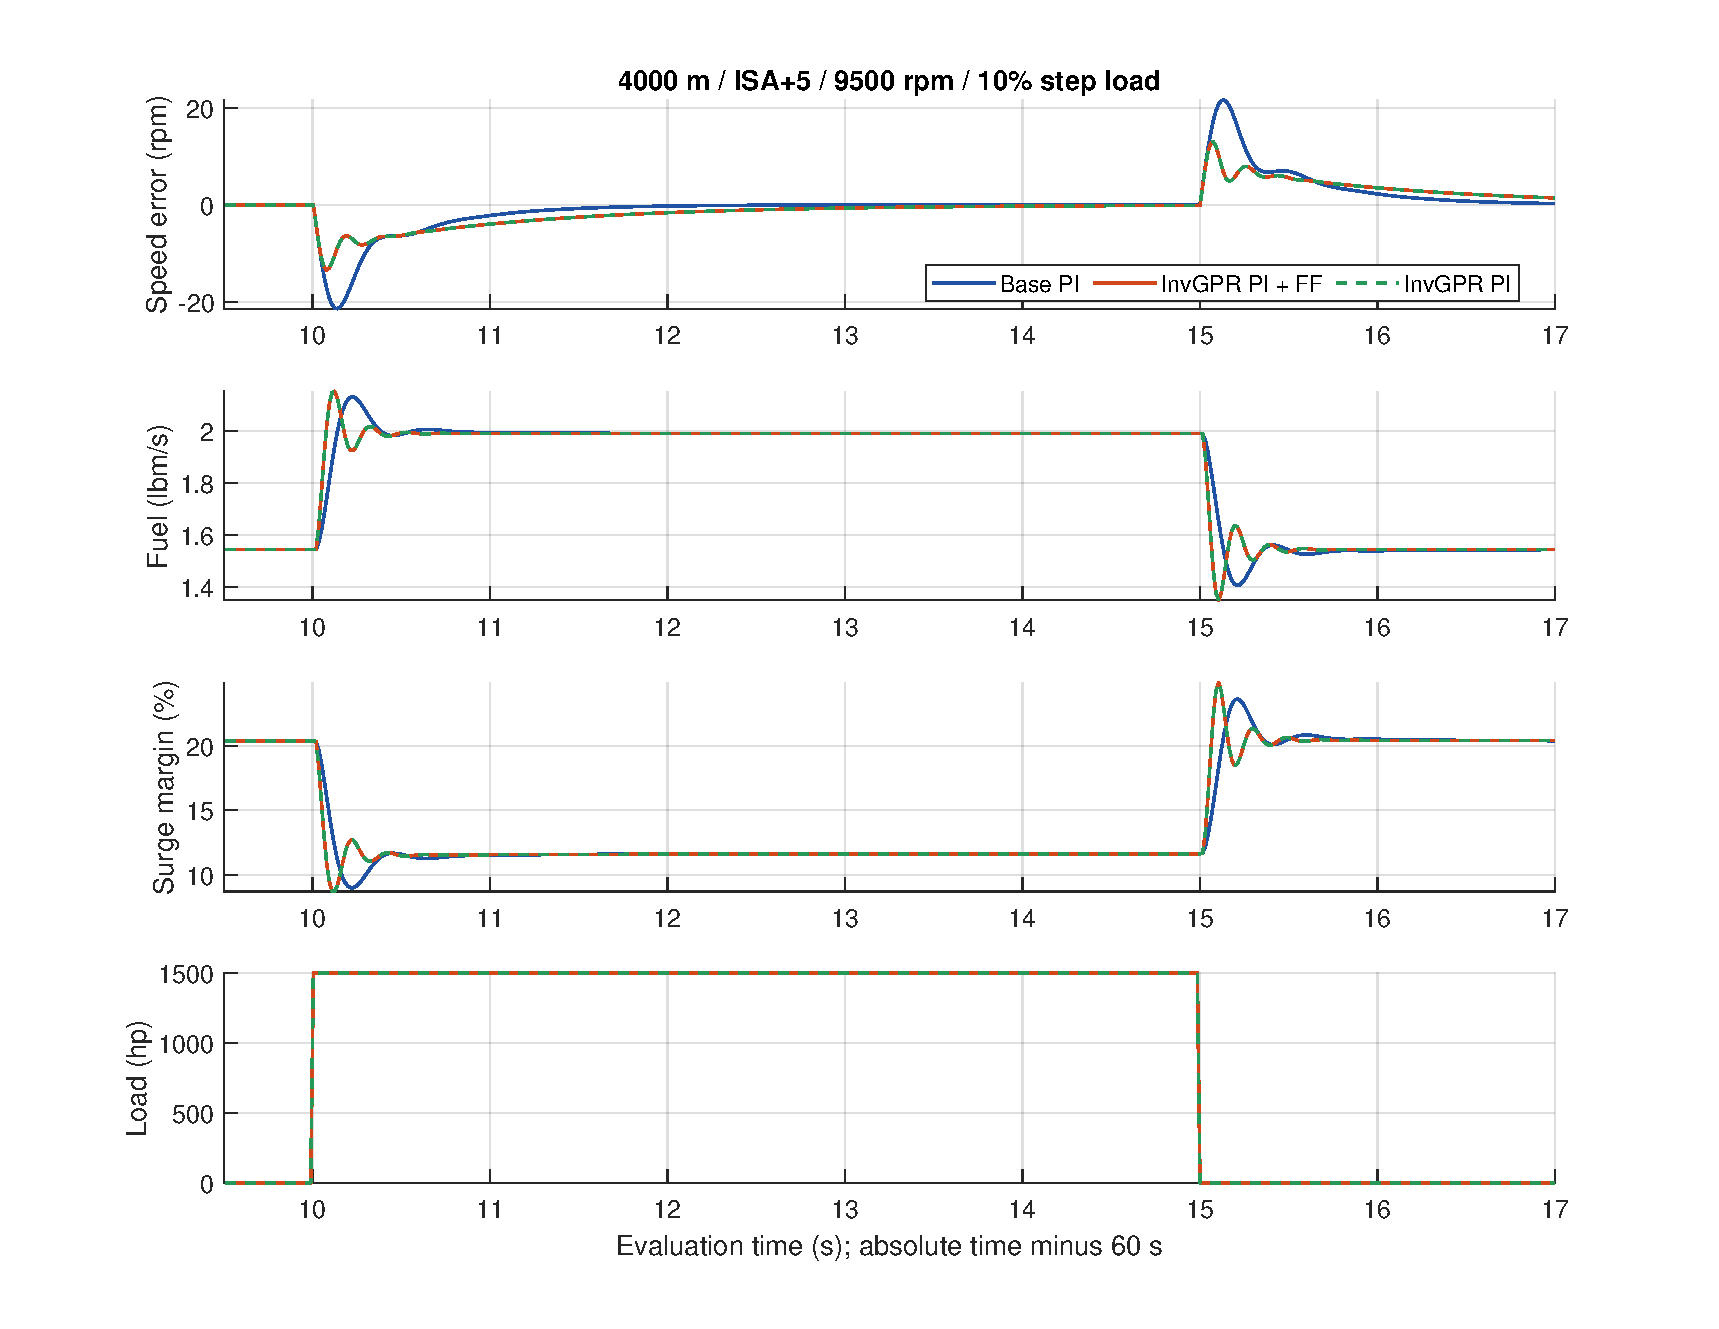
\includegraphics[width=\linewidth]{target_zoom_first.pdf}\caption{First 10\% load application and removal. The detailed fuel trace reveals reversals that are less apparent in the speed response.}\end{figure}

Application initially removes shaft power; unloading produces the opposite torque imbalance. The response must therefore be judged in both directions. The speed sensor and filtered acceleration delay and smooth the feedback motion signal, while the inverse sensitivity converts it into a virtual-fuel error. The fuel-reversal metric quantifies the reversals visible in this zoom without counting a simple monotonic fuel adjustment as ringing.

\clearpage
\subsection{Second load pulse}
\begin{figure}[H]\centering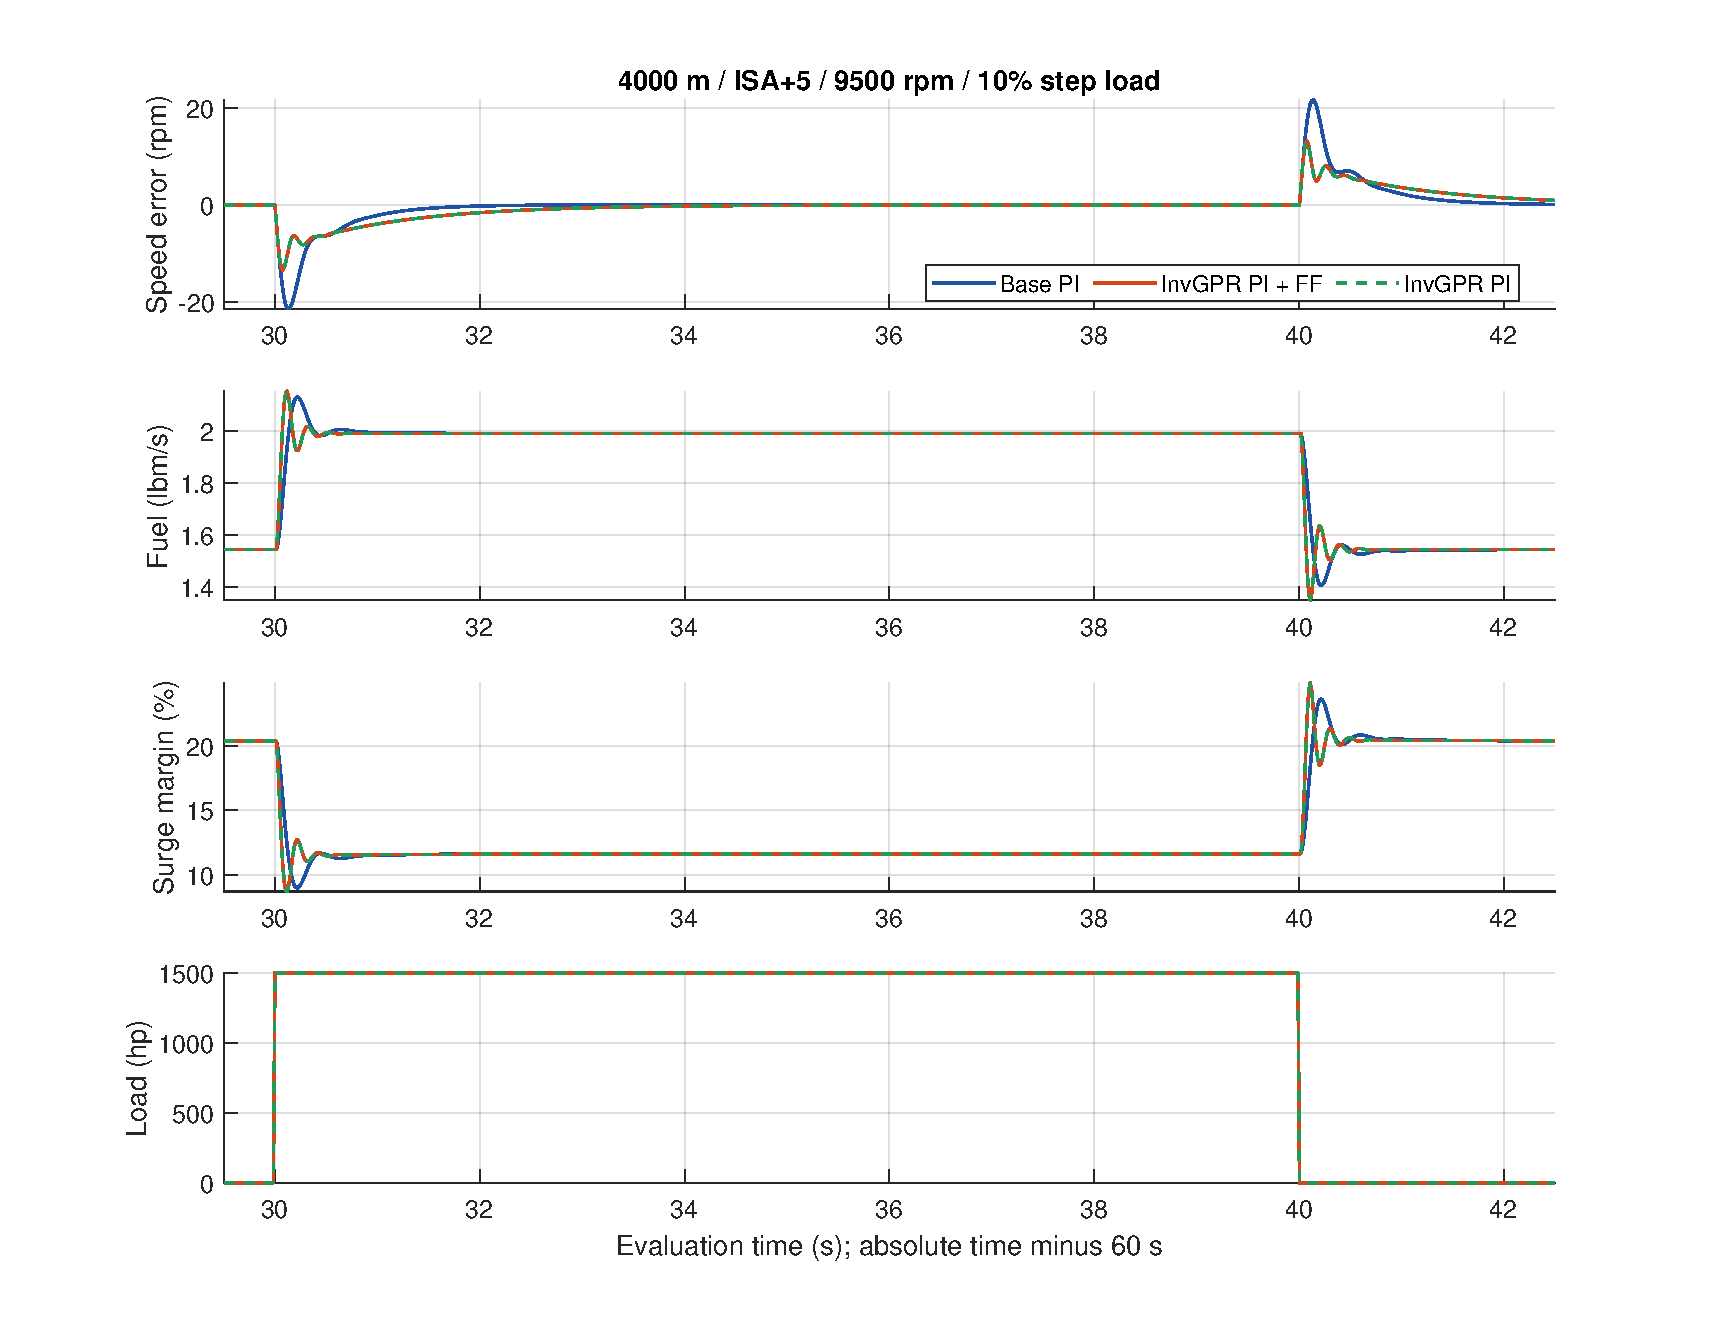
\includegraphics[width=\linewidth]{target_zoom_second.pdf}\caption{Second load pulse and its recovery. The same frozen gains and inverse posterior are used throughout.}\end{figure}

This window includes a longer dwell under the same load. Under a constant disturbance, the integral term supplies the fuel residual missing from the unloaded inverse model. Recovery measured from the unloading edge must not include a later load pulse. The event table uses the exact event boundaries to keep these intervals separate.

\clearpage
\subsection{Longest pulse and repeated recovery}
\begin{figure}[H]\centering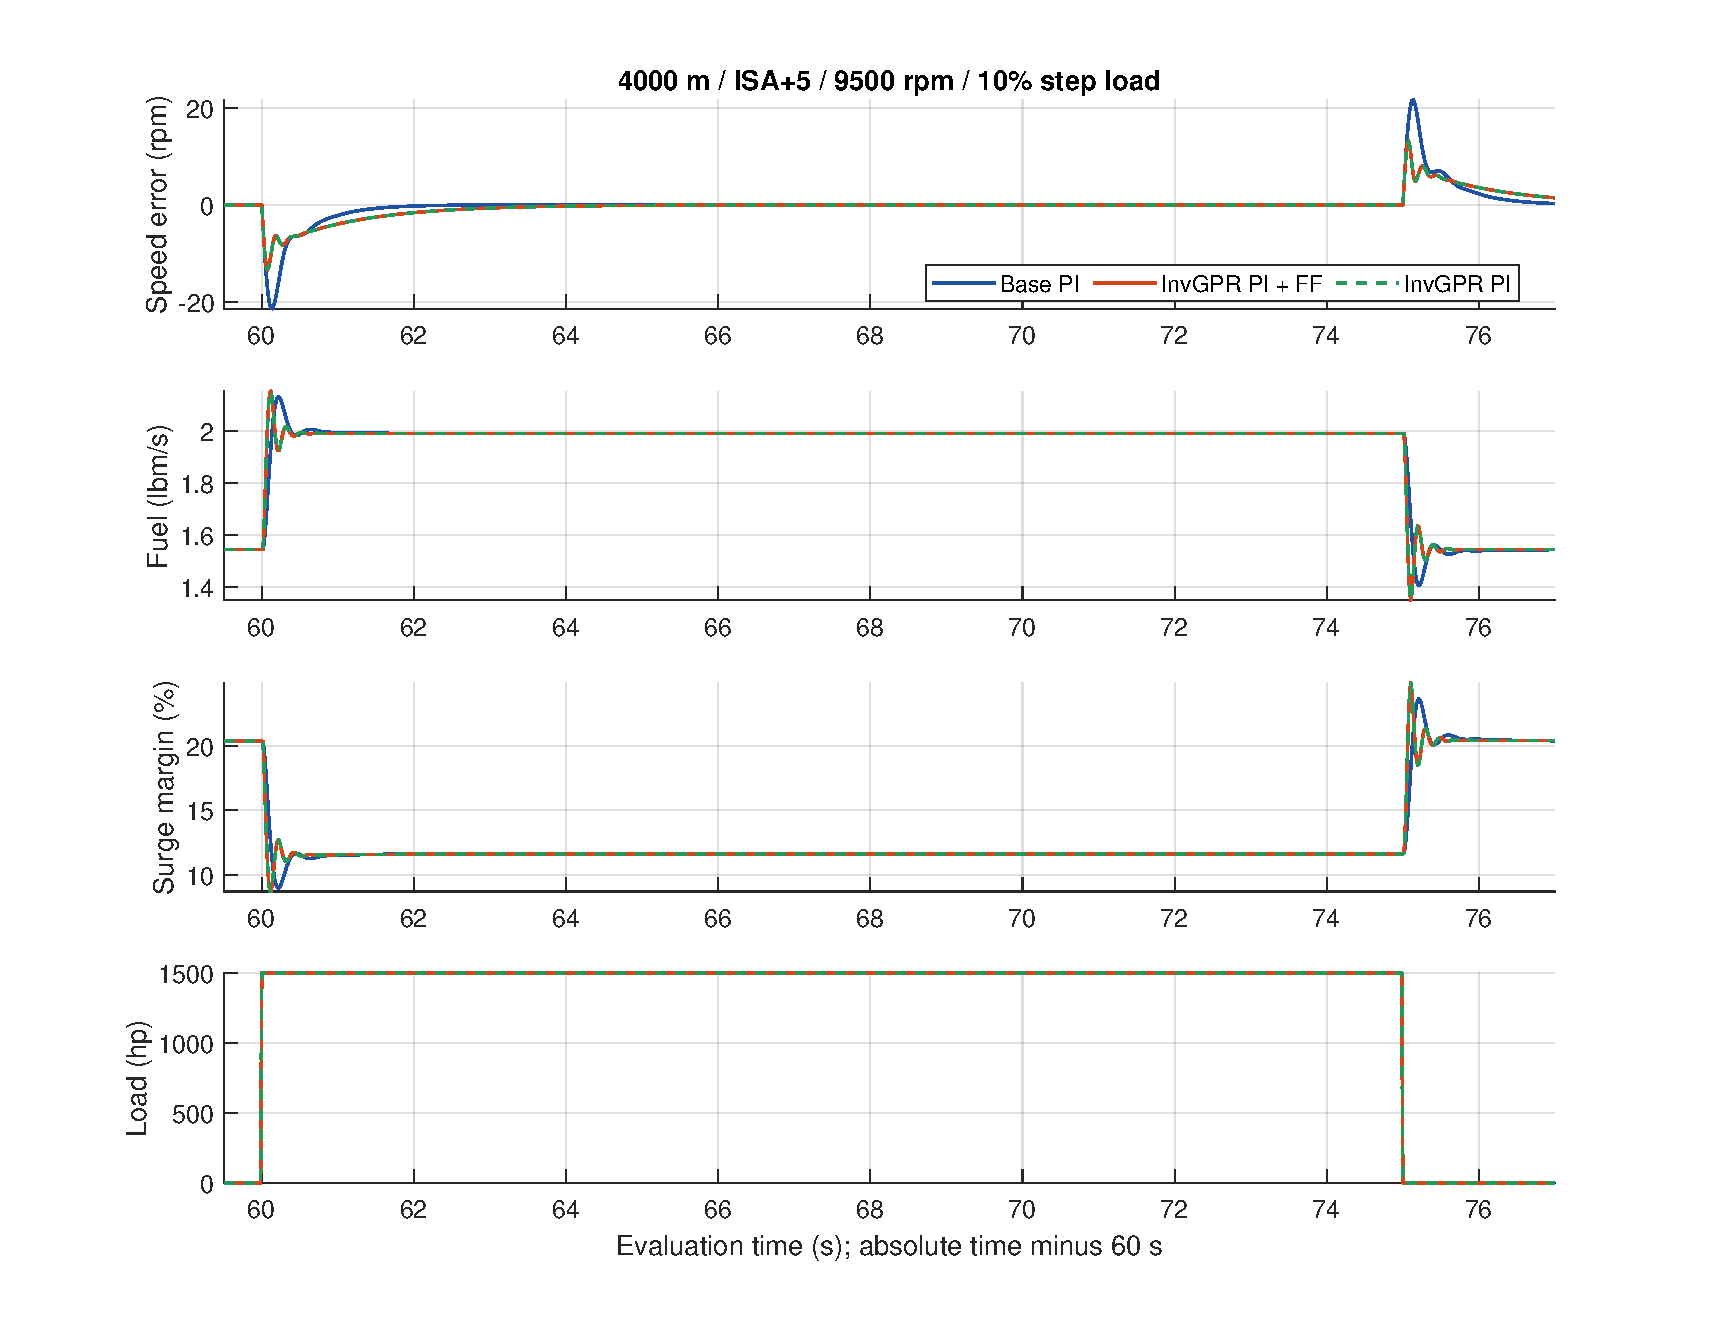
\includegraphics[width=\linewidth]{target_zoom_third.pdf}\caption{Third, longest load pulse. This window exposes sustained behaviour and unloading recovery.}\end{figure}

The final pulse checks whether the behaviour persists after repeated application and removal. It is still a finite-duration deterministic test; it does not establish robustness to noise, delays, unmodeled actuators or arbitrary loads.

\clearpage
\subsection{Event-level and internal controller evidence}
\begin{table}[H]\centering\small
\setlength{\tabcolsep}{5pt}
\begin{tabular}{@{}lrrrrrrr@{}}\toprule
Time (s) & Edge & Peak P & Peak VF & Ring P & Ring VF & $t_{.1}$ P & $t_{.1}$ VF\\\midrule
10.005 & on & 21.4 & 13.4 & 0.328 & 0.547 & 2.42 & NR\\
15 & off & 21.6 & 13 & 0.348 & 0.725 & 2.46 & 4.96\\
30 & on & 21.4 & 13.4 & 0.328 & 0.547 & 2.41 & 5.1\\
40.005 & off & 21.6 & 13.1 & 0.348 & 0.725 & 2.46 & 4.98\\
60 & on & 21.4 & 13.4 & 0.328 & 0.547 & 2.41 & 5.1\\
75 & off & 21.6 & 13.1 & 0.348 & 0.725 & 2.46 & 4.98\\
\bottomrule\end{tabular}\caption{Six individual load transitions. Peak errors are rpm, ringing is lbm/s, and supplementary recovery is seconds. Time is measured from the start of the 90 s evaluation.}\end{table}

\begin{figure}[H]\centering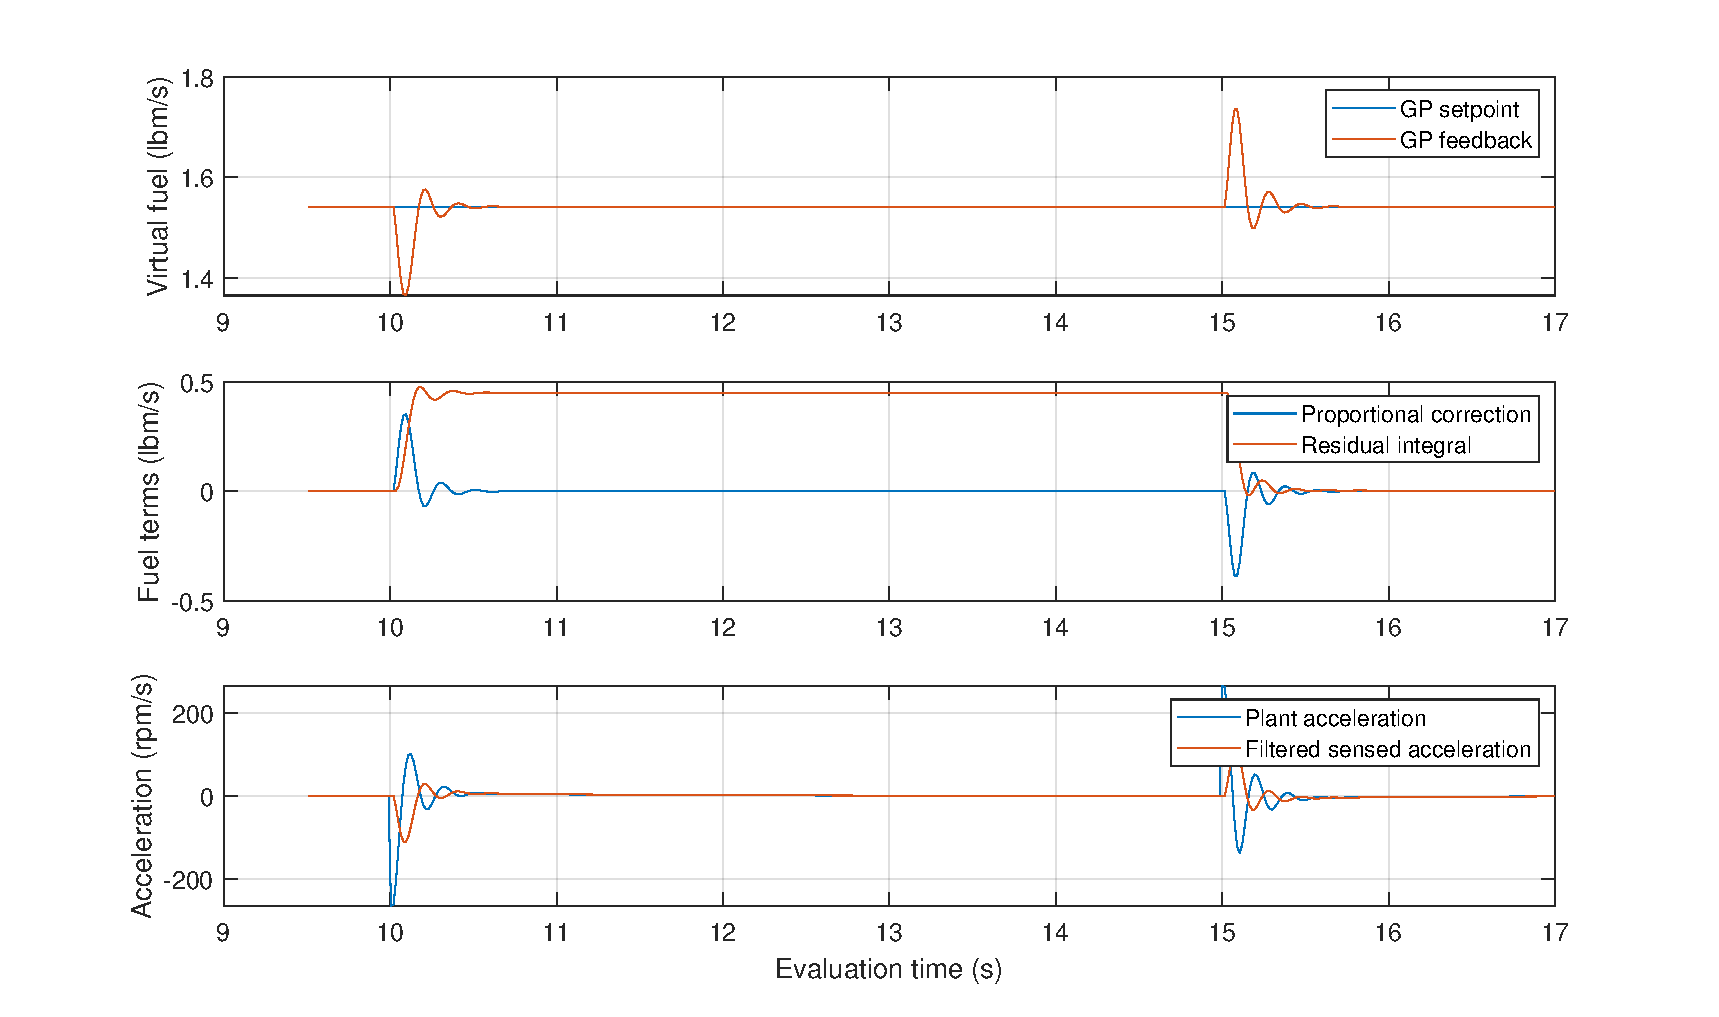
\includegraphics[width=\linewidth]{target_components.pdf}\caption{Virtual-fuel setpoint and feedback, PI correction terms, and plant versus estimated acceleration around the first pulse.}\end{figure}

The setpoint GP supplies nominal fuel for zero acceleration. The feedback GP maps filtered measured motion to virtual fuel. Their difference drives the proportional correction and residual integral. The derivative-like channel explains why apparently modest speed deviations can produce faster fuel motion. Direct plant acceleration is shown only for diagnosis and is not used as an online controller input.

Finite differences of the frozen posterior at the requested setpoint give $g_N=0.001458$ lbm/s per rpm and $g_a=0.001579$ lbm/s per (rpm/s). The ideal local equivalent proportional coefficient is 0.05027, the integral coefficient is 0.04373, and the derivative coefficient is 0.00316, in the corresponding speed-domain units. These are an interpretation of the inverse slopes, not a replacement controller. When the virtual error is close to zero, the local relation gives a speed-error tail with time constant $g_a/g_N\simeq1.083$ s. This helps explain the longer fine-settling tail despite the lower peak speed deviation.

\clearpage
\section{Performance across the 35-condition grid}
\begin{table}[H]\centering\small
\setlength{\tabcolsep}{5pt}
\begin{tabular}{@{}lrrrrrr@{}}\toprule
Method & Runs & Accepted & Map flag & Both checks & Median RMSE & Median ring\\\midrule
Base PI & 35 & 35 & 10 & 25 & 2.01 & 1.85\\
InvGPR PI + FF & 35 & 35 & 10 & 25 & 2.11 & 3.2\\
\bottomrule\end{tabular}\caption{Grid summary. Accepted uses solver, positivity, surge margin, finite signals and pre-disturbance trim. Both checks additionally requires the monitored compressor corrected speed to remain inside its map during evaluation. Medians use accepted runs and are not a paired comparison.}\end{table}

Both methods pass in 35 of the 35 grid environments. On these shared accepted cases, the inverse controller has lower RMSE in 18 cases and lower fuel ringing in 0 cases. Comparisons exclude rejected full runs from both sides, rather than averaging their valid prefixes.

The following tables report every requested altitude/ISA combination. P denotes base PI and VF denotes inverse-GPR PI plus feedforward. RMSE is in rpm, ringing in lbm/s, recovery in seconds and minimum surge margin in percent. A dash is a rejected full run, not missing execution. Asterisks identify compressor corrected-speed map overruns during evaluation, even if the numerical scores remain finite.

\begin{table}[H]\centering\small
\setlength{\tabcolsep}{5pt}
\begin{tabular}{@{}lrrrrrrrr@{}}\toprule
ISA & RMSE P & RMSE VF & Ring P & Ring VF & $t_{1\%}$ P & $t_{1\%}$ VF & SM P & SM VF\\\midrule
-30 & 4.53 & 3.58 & 3.7 & 6.8 & 0 & 0 & 6.68 & 6.58\\
-20 & 4.01 & 2.38 & 2.87 & 6.38 & 0 & 0 & 9.5 & 8.88\\
-10 & 3.53 & 2.09 & 2.55 & 5.6 & 0 & 0 & 12.5 & 11.7\\
+0 & 3.08 & 1.94 & 2.37 & 4.8 & 0 & 0 & 15.2 & 14.6\\
+10 & 2.72 & 1.79 & 2.17 & 4.3 & 0 & 0 & 17.1 & 16.5\\
+20 & 2.35 & 1.58 & 1.93 & 3.77 & 0 & 0 & 19.1 & 18.5\\
+30 & 2 & 1.38 & 1.73 & 3.2 & 0 & 0 & 21.6 & 21.1\\
\bottomrule\end{tabular}\caption{0 m: 9500 rpm and 10\% shaft-load steps. Units: RMSE rpm; ringing lbm/s; recovery s; SM percent. A dash means a rejected full run. An asterisk flags a compressor corrected-speed map overrun during evaluation.}\end{table}

\begin{table}[H]\centering\small
\setlength{\tabcolsep}{5pt}
\begin{tabular}{@{}lrrrrrrrr@{}}\toprule
ISA & RMSE P & RMSE VF & Ring P & Ring VF & $t_{1\%}$ P & $t_{1\%}$ VF & SM P & SM VF\\\midrule
-30 & 3.58 & 3.17 & 3.07 & 5.26 & 0 & 0 & 3.21 & 3.17\\
-20 & 3.46 & 3.06 & 2.96 & 5.15 & 0 & 0 & 5.31 & 5.35\\
-10 & 3.22 & 2.15 & 2.46 & 5.1 & 0 & 0 & 7.62 & 7.24\\
+0 & 2.88 & 1.95 & 2.25 & 4.36 & 0 & 0 & 10.5 & 10\\
+10 & 2.52 & 1.73 & 2 & 3.78 & 0 & 0 & 13.4 & 12.9\\
+20 & 2.21 & 1.65 & 1.85 & 3.28 & 0 & 0 & 15.9 & 15.5\\
+30 & 1.94 & 1.46 & 1.65 & 2.95 & 0 & 0 & 17.7 & 17.3\\
\bottomrule\end{tabular}\caption{2500 m: 9500 rpm and 10\% shaft-load steps. Units: RMSE rpm; ringing lbm/s; recovery s; SM percent. A dash means a rejected full run. An asterisk flags a compressor corrected-speed map overrun during evaluation.}\end{table}

\clearpage

\begin{table}[H]\centering\small
\setlength{\tabcolsep}{5pt}
\begin{tabular}{@{}lrrrrrrrr@{}}\toprule
ISA & RMSE P & RMSE VF & Ring P & Ring VF & $t_{1\%}$ P & $t_{1\%}$ VF & SM P & SM VF\\\midrule
-30$^*$ & 2.58 & 40.9 & 2.64 & 3.29 & 0 & NR & 2.03 & 2.39\\
-20$^*$ & 2.71 & 3.95 & 2.55 & 3.72 & 0 & 0 & 1.77 & 1.86\\
-10 & 2.58 & 2.62 & 2.28 & 3.73 & 0 & 0 & 3.93 & 3.98\\
+0 & 2.49 & 2.57 & 2.19 & 3.59 & 0 & 0 & 5.98 & 6.05\\
+10 & 2.27 & 1.75 & 1.85 & 3.39 & 0 & 0 & 8.55 & 8.34\\
+20 & 2.01 & 1.55 & 1.66 & 2.92 & 0 & 0 & 11.6 & 11.3\\
+30 & 1.75 & 1.38 & 1.49 & 2.53 & 0 & 0 & 14.4 & 14.2\\
\bottomrule\end{tabular}\caption{5000 m: 9500 rpm and 10\% shaft-load steps. Units: RMSE rpm; ringing lbm/s; recovery s; SM percent. A dash means a rejected full run. An asterisk flags a compressor corrected-speed map overrun during evaluation.}\end{table}

\begin{table}[H]\centering\small
\setlength{\tabcolsep}{5pt}
\begin{tabular}{@{}lrrrrrrrr@{}}\toprule
ISA & RMSE P & RMSE VF & Ring P & Ring VF & $t_{1\%}$ P & $t_{1\%}$ VF & SM P & SM VF\\\midrule
-30$^*$ & 1.65 & 22.2 & 1.81 & 2.25 & 0 & 0 & 2.83 & 3.2\\
-20$^*$ & 1.76 & 14.1 & 1.84 & 2.3 & 0 & 0 & 2.35 & 2.71\\
-10$^*$ & 1.86 & 31.1 & 1.87 & 2.42 & 0 & 0 & 1.86 & 2.22\\
+0 & 1.87 & 2.11 & 1.7 & 2.65 & 0 & 0 & 2.52 & 2.6\\
+10 & 1.81 & 2.11 & 1.63 & 2.56 & 0 & 0 & 4.66 & 4.76\\
+20 & 1.74 & 1.86 & 1.56 & 2.53 & 0 & 0 & 6.69 & 6.68\\
+30 & 1.55 & 1.41 & 1.33 & 2.23 & 0 & 0 & 9.53 & 9.46\\
\bottomrule\end{tabular}\caption{7500 m: 9500 rpm and 10\% shaft-load steps. Units: RMSE rpm; ringing lbm/s; recovery s; SM percent. A dash means a rejected full run. An asterisk flags a compressor corrected-speed map overrun during evaluation.}\end{table}

\begin{table}[H]\centering\small
\setlength{\tabcolsep}{5pt}
\begin{tabular}{@{}lrrrrrrrr@{}}\toprule
ISA & RMSE P & RMSE VF & Ring P & Ring VF & $t_{1\%}$ P & $t_{1\%}$ VF & SM P & SM VF\\\midrule
-30$^*$ & 1.05 & 4.96 & 1.25 & 1.38 & 0 & 0 & 3.44 & 4\\
-20$^*$ & 1.11 & 6.85 & 1.25 & 1.52 & 0 & 0 & 3.12 & 3.54\\
-10$^*$ & 1.17 & 7.11 & 1.26 & 1.58 & 0 & 0 & 2.66 & 3.01\\
+0$^*$ & 1.25 & 6.26 & 1.28 & 1.63 & 0 & 0 & 2.17 & 2.54\\
+10$^*$ & 1.32 & 21.7 & 1.3 & 1.74 & 0 & 0 & 1.67 & 2.01\\
+20 & 1.29 & 1.7 & 1.19 & 1.79 & 0 & 0 & 3.29 & 3.43\\
+30 & 1.24 & 1.64 & 1.14 & 1.73 & 0 & 0 & 5.37 & 5.51\\
\bottomrule\end{tabular}\caption{10000 m: 9500 rpm and 10\% shaft-load steps. Units: RMSE rpm; ringing lbm/s; recovery s; SM percent. A dash means a rejected full run. An asterisk flags a compressor corrected-speed map overrun during evaluation.}\end{table}


Among the 25 conditions without a monitored compressor corrected-speed overrun, inverse GPR lowers RMSE in 18 cases. It has higher fuel ringing than base PI in every one of the 35 conditions. Thus the new inputs improve environmental representation but the fixed gains do not deliver a fuel-smoothness advantage. The worst inverse RMSE is 40.90 rpm at 5000 m/ISA-30, compared with 2.58 rpm for base PI; that map-flagged inverse run also fails the requested 1\% recovery criterion in at least one event. All base-PI grid runs remain inside the 1\% band throughout.

\clearpage
\subsection{Accuracy and ringing across the envelope}
\begin{figure}[H]\centering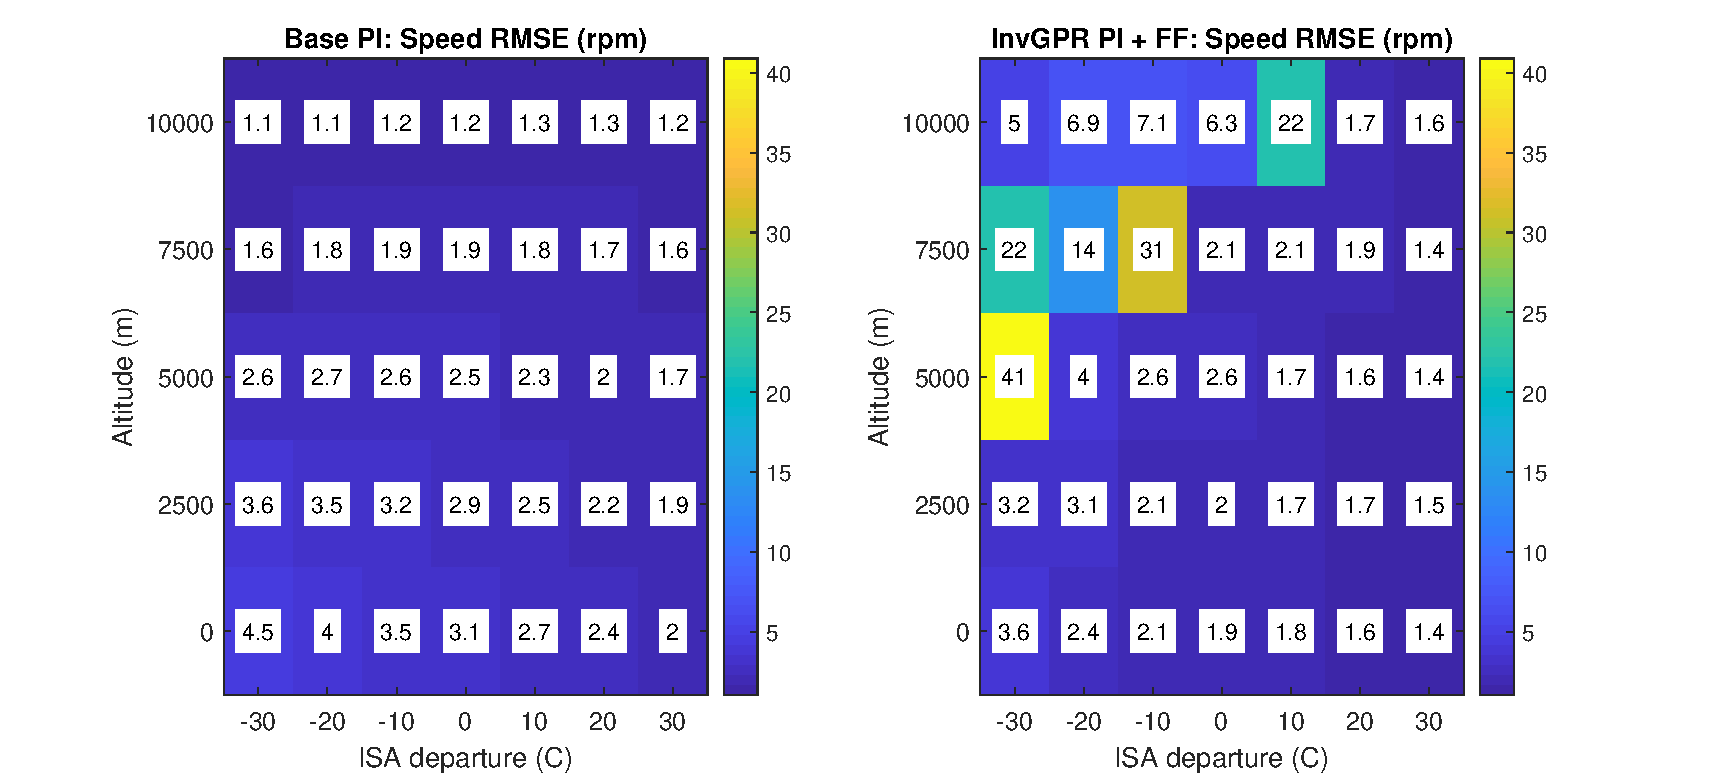
\includegraphics[width=\linewidth]{grid_rmse_rpm.pdf}\caption{Speed RMSE over the 35 environmental combinations. Grey cells marked X are rejected full runs. Both panels use the same colour scale.}\end{figure}

\begin{figure}[H]\centering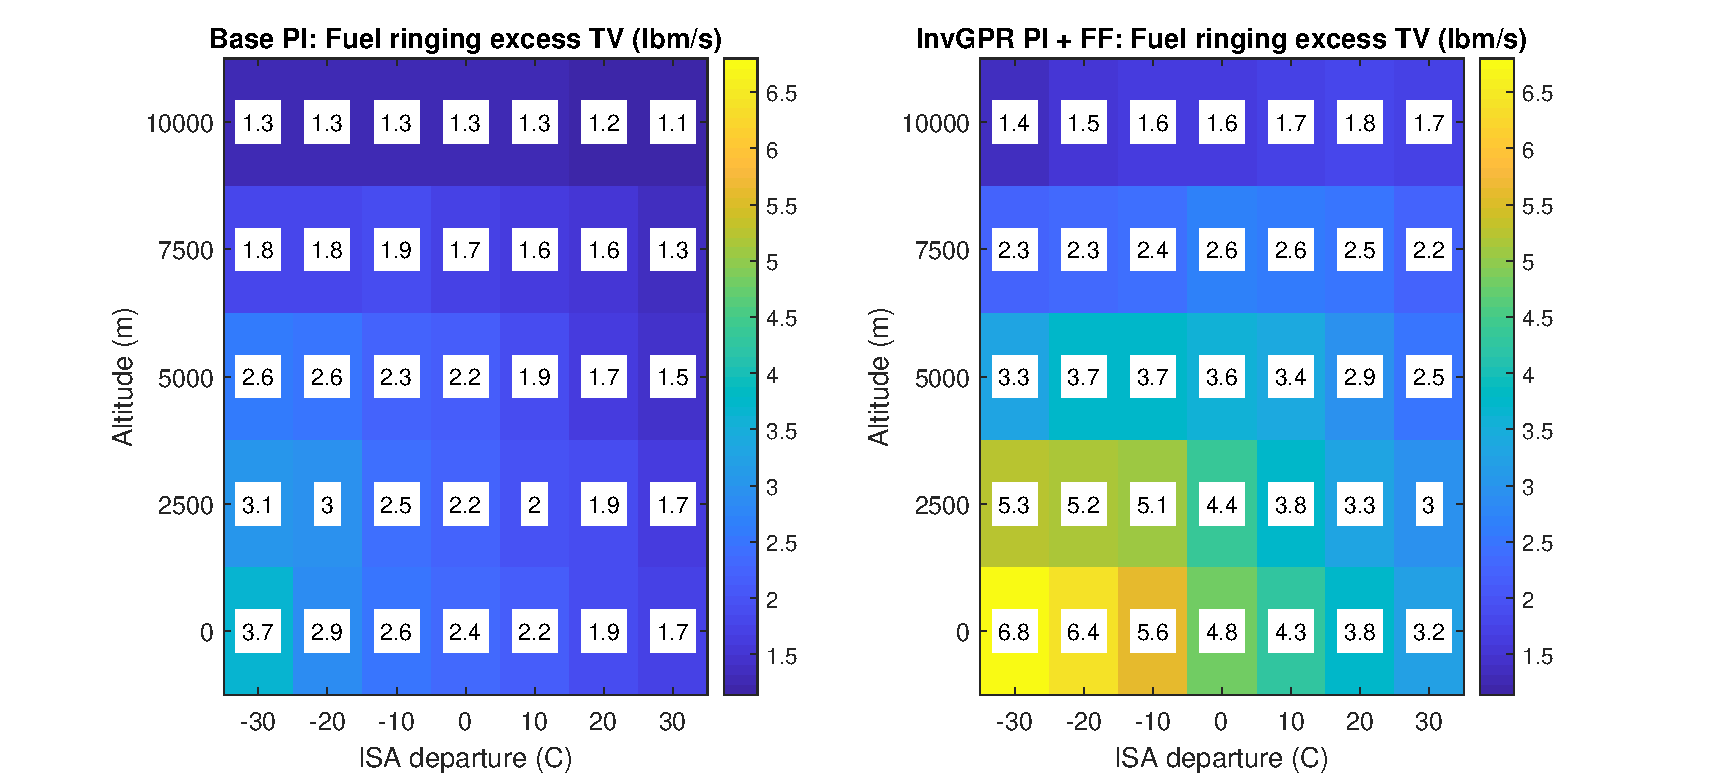
\includegraphics[width=\linewidth]{grid_ringing_excess_TV_lbm_s.pdf}\caption{Fuel-ringing score over the grid. These heatmaps do not themselves encode compressor map support; use the flagged tables.}\end{figure}

The common colour scales permit a direct visual comparison within each metric. The paired counts above avoid mistaking different failure sets for a performance advantage. A lower ringing score is not sufficient when the same run fails surge or solver validity, and a finite numerical score in a map-flagged condition remains a simulator-only result.

\clearpage
\subsection{Recovery across the envelope}
\begin{figure}[H]\centering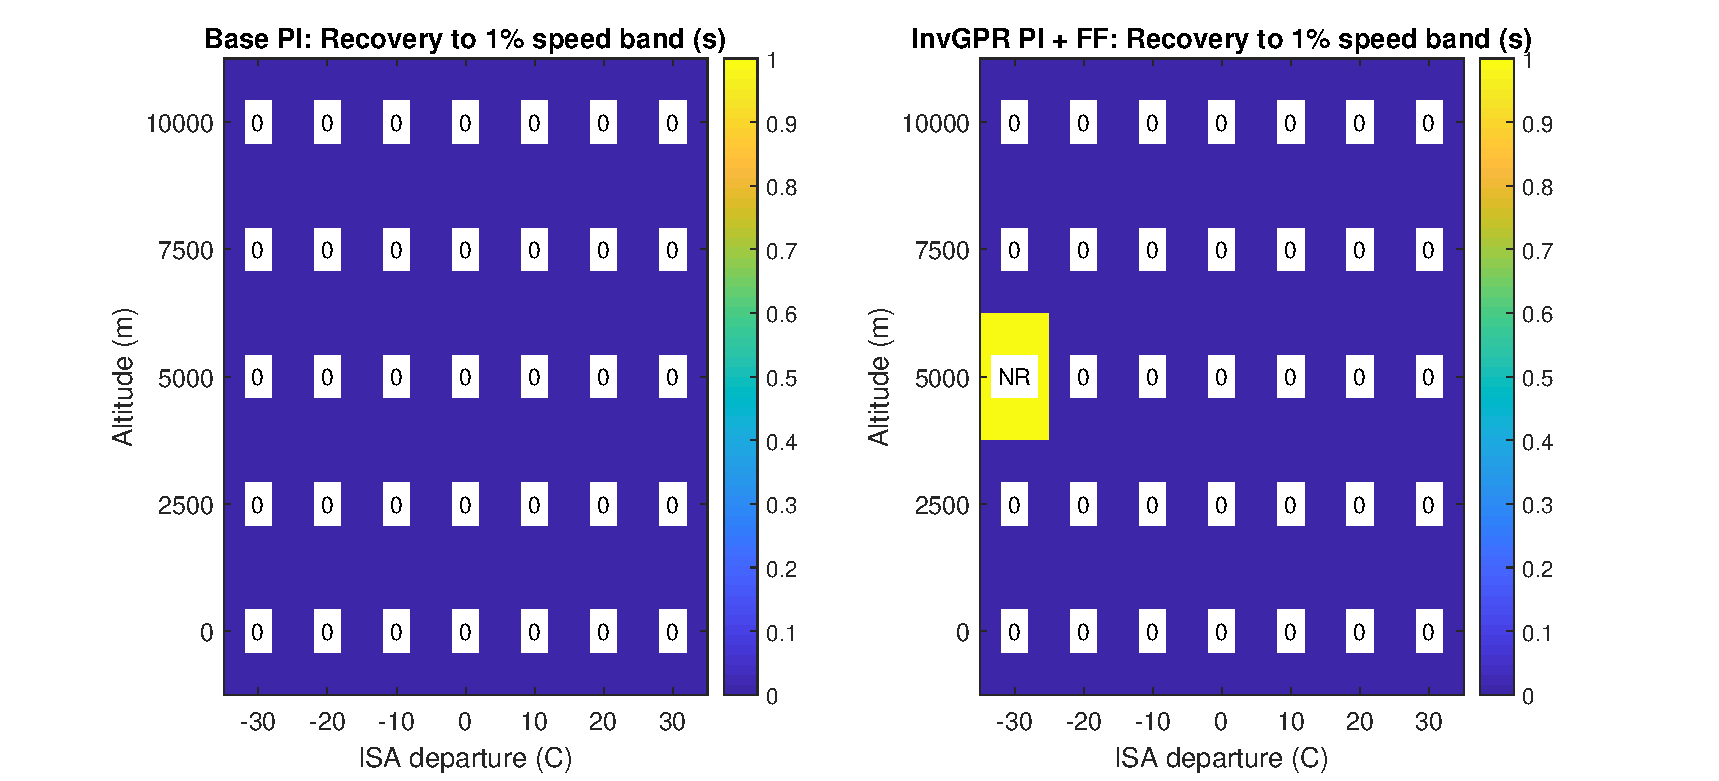
\includegraphics[width=\linewidth]{grid_recovery_1pct_speed_s.pdf}\caption{Requested 1\% speed-band recovery. Zero denotes no excursion beyond the band, not instantaneous or perfect speed tracking.}\end{figure}

\begin{figure}[H]\centering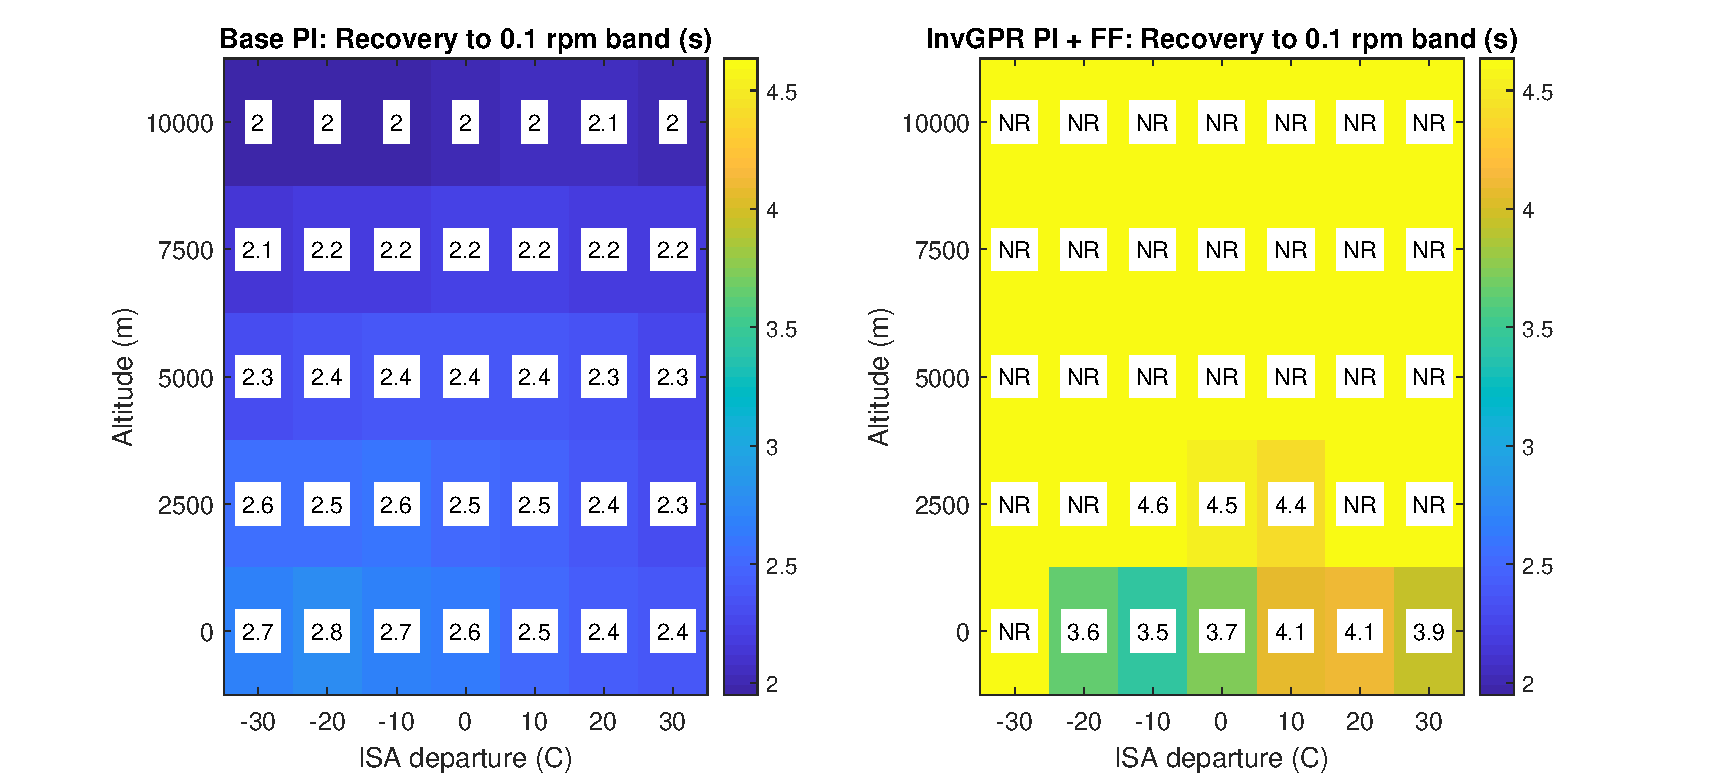
\includegraphics[width=\linewidth]{grid_settling_to_point1_rpm_s.pdf}\caption{Supplementary recovery to a 0.1 rpm band. This tighter measure can distinguish transients that stay within the 1\% band.}\end{figure}

The 1\% and 0.1 rpm bands answer different questions. The former tests whether speed remains close to its nominal operating value in relative terms; the latter tests the fine settling tail. The requested band can become non-discriminating without either controller being perfect.

\clearpage
\section{Failures, interpretation and practical limits}
All comparison trajectories passed the numerical criteria.
The grid extends beyond the original example's well-supported compressor regime in several cold/high-altitude conditions. The GP can learn the numerical boundary behaviour of the supplied plant, but it cannot manufacture missing compressor-map information. The flagged training and test counts, the two unavailable held-out conditions, and the late speed-band violation must accompany any aggregate performance claim.

The environmental extension resolves an important missing-input problem, but it does not make the inverse globally unique. Shaft load, hidden states, component deterioration and actuator dynamics are not inverse inputs. Their effects must be handled by feedback or by a richer model. Retaining fixed gains is the requested transfer test; it deliberately does not guarantee equal damping across environments because both the plant and inverse derivatives vary.

The 4000 m/ISA+5 comparison is the most direct evidence for the requested use case. Generalization to the full grid should additionally require adequate component-map coverage. Future gain or model changes should be evaluated on fresh validation trajectories rather than repeatedly optimized on the 200 frozen test observations.

\begin{figure}[H]\centering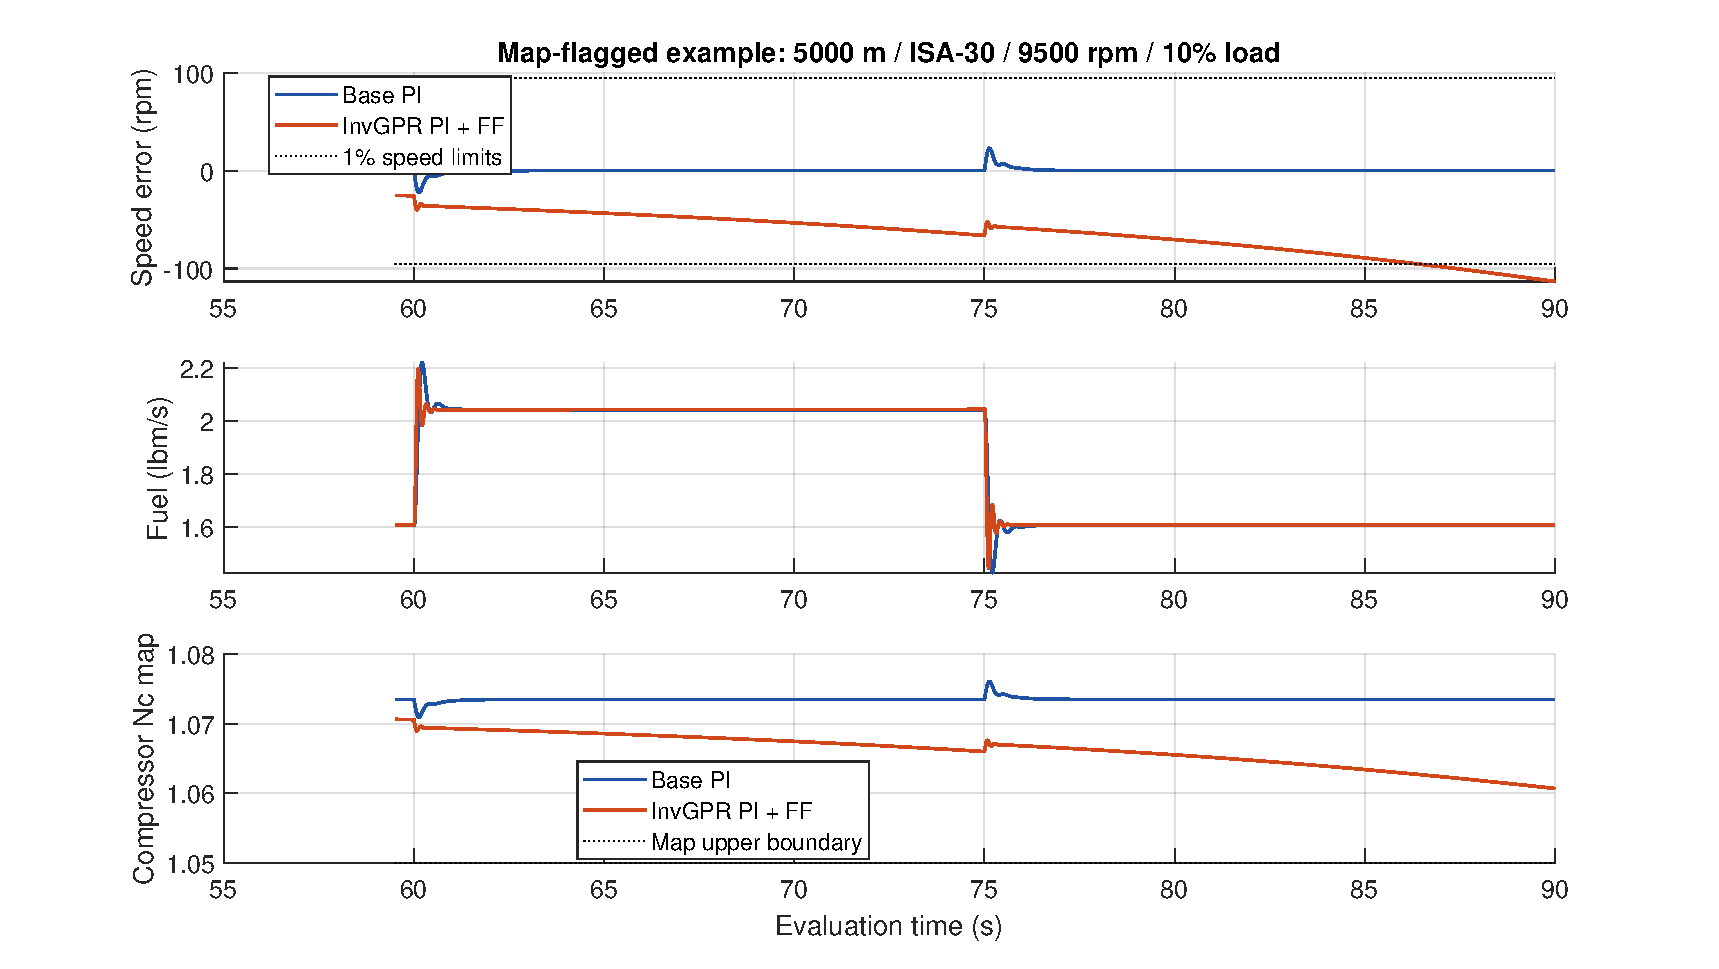
\includegraphics[width=\linewidth]{grid_worst_zoom.pdf}\caption{A map-flagged grid example: inverse-controller speed drifts outside the 1\% band late in the final unloaded interval and does not recover by the end of evaluation. Numerical convergence is insufficient as a tracking-performance criterion.}\end{figure}


\clearpage
\section{Reproduction and deliverables}
The complete source study is stored in \path{results/environment\_gpr\_20260914\_201325}. Its principal records are the 35 \path{environment_XX.mat} identification trajectories, the frozen \path{environment_inverse_gpr_model.mat}, the training and 200-point test tables, condition-specific unloaded trim records, and all 73 comparison MAT/CSV trajectories.

\begin{enumerate}
\item \path{run_tmats_environment_data.m} generates the 35 unloaded identification/held-out trajectories. \path{tmats_environment_config.m} defines units and preparation; \path{tmats_environment_patch.m} adds temperature departure to the existing plant in memory.
\item \path{fit_tmats_environment_gpr.m} selects 1,400 training points, fits exact GPR, freezes it, and validates exactly 200 held-out samples. An existing frozen model is reused rather than refitted during validation.
\item \path{run_tmats_environment_comparison.m} runs each trim and comparison with unchanged gains. \path{tmats_environment_vf_sfun.m} implements the six-input controller; \path{predict_tmats_environment_gpr.m} provides mean and standard-deviation predictions.
\item \path{report_tmats_environment_study.m} exports the numerical summary, event metrics and vector figures. \path{build_tmats_environment_report.py} inserts measured results into the LaTeX source. Run \texttt{pdflatex} twice on \path{Environment_Controller_Tutorial.tex} to rebuild the PDF.
\end{enumerate}
The original saved controller models are preserved; the new interfaces are applied to isolated in-memory copies for the study. A dedicated \path{GasTurbine_Dyn_EnvironmentGPR.mdl} is also supplied, with \path{tmats_environment_controller_setup.m} loading the target case and frozen gains. The LaTeX package includes the figure PDFs and numerical tables so rebuilding the report does not require rerunning Simulink. MATLAB R2018b, T-MATS and the Statistics and Machine Learning Toolbox are required to repeat fitting and simulation.

\begin{thebibliography}{9}
\bibitem{gpml} C. E. Rasmussen and C. K. I. Williams, \emph{Gaussian Processes for Machine Learning}, MIT Press, 2006, Chapter 2. \url{https://gaussianprocess.org/gpml/chapters/RW2.pdf}.
\bibitem{mathworks} MathWorks, \emph{fitrgp: Fit a Gaussian process regression model}; exact fit/prediction and ARD squared-exponential covariance. \url{https://www.mathworks.com/help/stats/fitrgp.html}.
\bibitem{tmats} J. W. Chapman et al., \emph{Toolbox for the Modeling and Analysis of Thermodynamic Systems (T-MATS) User's Guide}, NASA/TM-2014-216638. \url{https://ntrs.nasa.gov/archive/nasa/casi.ntrs.nasa.gov/20140012486.pdf}.
\end{thebibliography}
\end{document}
